\PassOptionsToPackage{unicode=true}{hyperref} % options for packages loaded elsewhere
\PassOptionsToPackage{hyphens}{url}
%
\documentclass[]{article}
\usepackage{lmodern}
\usepackage{amssymb,amsmath}
\usepackage{ifxetex,ifluatex}
\usepackage{fixltx2e} % provides \textsubscript
\ifnum 0\ifxetex 1\fi\ifluatex 1\fi=0 % if pdftex
  \usepackage[T1]{fontenc}
  \usepackage[utf8]{inputenc}
  \usepackage{textcomp} % provides euro and other symbols
\else % if luatex or xelatex
  \usepackage{unicode-math}
  \defaultfontfeatures{Ligatures=TeX,Scale=MatchLowercase}
\fi
% use upquote if available, for straight quotes in verbatim environments
\IfFileExists{upquote.sty}{\usepackage{upquote}}{}
% use microtype if available
\IfFileExists{microtype.sty}{%
\usepackage[]{microtype}
\UseMicrotypeSet[protrusion]{basicmath} % disable protrusion for tt fonts
}{}
\IfFileExists{parskip.sty}{%
\usepackage{parskip}
}{% else
\setlength{\parindent}{0pt}
\setlength{\parskip}{6pt plus 2pt minus 1pt}
}
\usepackage{hyperref}
\hypersetup{
            pdftitle={Term Project},
            pdfauthor={Leslie Speight Youtsey and Elizabeth Weatherup},
            pdfborder={0 0 0},
            breaklinks=true}
\urlstyle{same}  % don't use monospace font for urls
\usepackage[margin=1in]{geometry}
\usepackage{color}
\usepackage{fancyvrb}
\newcommand{\VerbBar}{|}
\newcommand{\VERB}{\Verb[commandchars=\\\{\}]}
\DefineVerbatimEnvironment{Highlighting}{Verbatim}{commandchars=\\\{\}}
% Add ',fontsize=\small' for more characters per line
\usepackage{framed}
\definecolor{shadecolor}{RGB}{248,248,248}
\newenvironment{Shaded}{\begin{snugshade}}{\end{snugshade}}
\newcommand{\AlertTok}[1]{\textcolor[rgb]{0.94,0.16,0.16}{#1}}
\newcommand{\AnnotationTok}[1]{\textcolor[rgb]{0.56,0.35,0.01}{\textbf{\textit{#1}}}}
\newcommand{\AttributeTok}[1]{\textcolor[rgb]{0.77,0.63,0.00}{#1}}
\newcommand{\BaseNTok}[1]{\textcolor[rgb]{0.00,0.00,0.81}{#1}}
\newcommand{\BuiltInTok}[1]{#1}
\newcommand{\CharTok}[1]{\textcolor[rgb]{0.31,0.60,0.02}{#1}}
\newcommand{\CommentTok}[1]{\textcolor[rgb]{0.56,0.35,0.01}{\textit{#1}}}
\newcommand{\CommentVarTok}[1]{\textcolor[rgb]{0.56,0.35,0.01}{\textbf{\textit{#1}}}}
\newcommand{\ConstantTok}[1]{\textcolor[rgb]{0.00,0.00,0.00}{#1}}
\newcommand{\ControlFlowTok}[1]{\textcolor[rgb]{0.13,0.29,0.53}{\textbf{#1}}}
\newcommand{\DataTypeTok}[1]{\textcolor[rgb]{0.13,0.29,0.53}{#1}}
\newcommand{\DecValTok}[1]{\textcolor[rgb]{0.00,0.00,0.81}{#1}}
\newcommand{\DocumentationTok}[1]{\textcolor[rgb]{0.56,0.35,0.01}{\textbf{\textit{#1}}}}
\newcommand{\ErrorTok}[1]{\textcolor[rgb]{0.64,0.00,0.00}{\textbf{#1}}}
\newcommand{\ExtensionTok}[1]{#1}
\newcommand{\FloatTok}[1]{\textcolor[rgb]{0.00,0.00,0.81}{#1}}
\newcommand{\FunctionTok}[1]{\textcolor[rgb]{0.00,0.00,0.00}{#1}}
\newcommand{\ImportTok}[1]{#1}
\newcommand{\InformationTok}[1]{\textcolor[rgb]{0.56,0.35,0.01}{\textbf{\textit{#1}}}}
\newcommand{\KeywordTok}[1]{\textcolor[rgb]{0.13,0.29,0.53}{\textbf{#1}}}
\newcommand{\NormalTok}[1]{#1}
\newcommand{\OperatorTok}[1]{\textcolor[rgb]{0.81,0.36,0.00}{\textbf{#1}}}
\newcommand{\OtherTok}[1]{\textcolor[rgb]{0.56,0.35,0.01}{#1}}
\newcommand{\PreprocessorTok}[1]{\textcolor[rgb]{0.56,0.35,0.01}{\textit{#1}}}
\newcommand{\RegionMarkerTok}[1]{#1}
\newcommand{\SpecialCharTok}[1]{\textcolor[rgb]{0.00,0.00,0.00}{#1}}
\newcommand{\SpecialStringTok}[1]{\textcolor[rgb]{0.31,0.60,0.02}{#1}}
\newcommand{\StringTok}[1]{\textcolor[rgb]{0.31,0.60,0.02}{#1}}
\newcommand{\VariableTok}[1]{\textcolor[rgb]{0.00,0.00,0.00}{#1}}
\newcommand{\VerbatimStringTok}[1]{\textcolor[rgb]{0.31,0.60,0.02}{#1}}
\newcommand{\WarningTok}[1]{\textcolor[rgb]{0.56,0.35,0.01}{\textbf{\textit{#1}}}}
\usepackage{graphicx,grffile}
\makeatletter
\def\maxwidth{\ifdim\Gin@nat@width>\linewidth\linewidth\else\Gin@nat@width\fi}
\def\maxheight{\ifdim\Gin@nat@height>\textheight\textheight\else\Gin@nat@height\fi}
\makeatother
% Scale images if necessary, so that they will not overflow the page
% margins by default, and it is still possible to overwrite the defaults
% using explicit options in \includegraphics[width, height, ...]{}
\setkeys{Gin}{width=\maxwidth,height=\maxheight,keepaspectratio}
\setlength{\emergencystretch}{3em}  % prevent overfull lines
\providecommand{\tightlist}{%
  \setlength{\itemsep}{0pt}\setlength{\parskip}{0pt}}
\setcounter{secnumdepth}{0}
% Redefines (sub)paragraphs to behave more like sections
\ifx\paragraph\undefined\else
\let\oldparagraph\paragraph
\renewcommand{\paragraph}[1]{\oldparagraph{#1}\mbox{}}
\fi
\ifx\subparagraph\undefined\else
\let\oldsubparagraph\subparagraph
\renewcommand{\subparagraph}[1]{\oldsubparagraph{#1}\mbox{}}
\fi

% set default figure placement to htbp
\makeatletter
\def\fps@figure{htbp}
\makeatother


\title{Term Project}
\author{Leslie Speight Youtsey and Elizabeth Weatherup}
\date{10/22/2020}

\begin{document}
\maketitle

\begin{Shaded}
\begin{Highlighting}[]
\NormalTok{bats_flux <-}\StringTok{ }\KeywordTok{read.csv}\NormalTok{(}\StringTok{"bats_flux.csv"}\NormalTok{)}

\NormalTok{delete.na <-}\StringTok{ }\ControlFlowTok{function}\NormalTok{(DF, }\DataTypeTok{n=}\DecValTok{0}\NormalTok{) \{}
\NormalTok{  DF[}\KeywordTok{rowSums}\NormalTok{(}\KeywordTok{is.na}\NormalTok{(DF)) }\OperatorTok{<=}\StringTok{ }\NormalTok{n,]}
\NormalTok{\} }\CommentTok{#Function that takes rows out that contains NAs }

\NormalTok{bats_flux.noNA <-}\StringTok{ }\KeywordTok{delete.na}\NormalTok{(bats_flux) }\CommentTok{# Take out rows containing NAs }


\NormalTok{Data <-}\StringTok{ }\KeywordTok{subset}\NormalTok{(bats_flux,}\DataTypeTok{select =} \KeywordTok{c}\NormalTok{(}\StringTok{"cr"}\NormalTok{,}\StringTok{"dep"}\NormalTok{,}\StringTok{"yymmdd1"}\NormalTok{,}\StringTok{"yymmdd2"}\NormalTok{,}\StringTok{"Lat2"}\NormalTok{,}\StringTok{"Lat2.1"}\NormalTok{,}\StringTok{"Long1"}\NormalTok{,}\StringTok{"Long2"}\NormalTok{,}\StringTok{"M_avg"}\NormalTok{,}\StringTok{"C_avg"}\NormalTok{,}\StringTok{"N_avg"}\NormalTok{,}\StringTok{"P_avg"}\NormalTok{))}

\NormalTok{Data.noNA <-}\StringTok{ }\KeywordTok{delete.na}\NormalTok{(Data)}

\CommentTok{#Data_noNA <- write.csv(x= Data.noNA,file = "Data_noNA.csv")}
\end{Highlighting}
\end{Shaded}

ANOVA Trial

\begin{Shaded}
\begin{Highlighting}[]
\CommentTok{#we want to make predictions on the Mass average flux. }

\CommentTok{# we want to compare this against depth and C,N,P fluxes }

\CommentTok{# Depth is categorical }
\CommentTok{# N,P,C are numerical }

\KeywordTok{library}\NormalTok{(psych) }\CommentTok{# for `pairs.panels()`}
\KeywordTok{library}\NormalTok{(lattice)}

\NormalTok{ANOCOVA.data <-}\StringTok{ }\KeywordTok{subset}\NormalTok{(Data.noNA, }\DataTypeTok{select =} \KeywordTok{c}\NormalTok{(}\StringTok{"dep"}\NormalTok{, }\StringTok{"M_avg"}\NormalTok{, }\StringTok{"C_avg"}\NormalTok{,}\StringTok{"N_avg"}\NormalTok{,}\StringTok{"P_avg"}\NormalTok{))}
\KeywordTok{as.character}\NormalTok{(ANOCOVA.data}\OperatorTok{$}\NormalTok{dep) }\CommentTok{# need to make dep categorical not numerical }
\end{Highlighting}
\end{Shaded}

\begin{verbatim}
##   [1] "150" "200" "300" "150" "200" "300" "150" "200" "300" "150" "200" "300"
##  [13] "150" "200" "300" "150" "200" "300" "150" "200" "300" "150" "200" "300"
##  [25] "150" "200" "300" "150" "200" "300" "150" "200" "300" "150" "200" "300"
##  [37] "150" "200" "300" "150" "200" "300" "150" "200" "300" "150" "200" "300"
##  [49] "150" "200" "300" "150" "200" "300" "150" "200" "300" "150" "200" "300"
##  [61] "150" "200" "300" "150" "200" "300" "150" "200" "300" "150" "200" "300"
##  [73] "150" "200" "300" "150" "200" "300" "150" "200" "300" "150" "200" "300"
##  [85] "150" "200" "300" "150" "200" "300" "150" "200" "300" "150" "200" "300"
##  [97] "150" "200" "300" "150" "150" "200" "300" "150" "200" "300" "150" "200"
## [109] "300" "150" "200" "300" "150" "200" "300" "150" "200" "300" "150" "200"
## [121] "300" "150" "200" "300" "150" "200" "300" "150" "200" "300" "150" "200"
## [133] "300" "150" "150" "200" "300" "150" "200" "300" "150" "200" "300" "150"
## [145] "200" "300" "150" "200" "300" "150" "200" "300" "150" "200" "300" "150"
## [157] "150" "200" "300" "150" "200" "300" "150" "200" "300" "150" "200" "300"
## [169] "150" "200" "300" "150" "200" "300" "150" "200" "300" "150" "200" "300"
## [181] "150" "200" "300" "150" "200" "300" "150" "200" "300" "150" "200" "300"
## [193] "150" "200" "300" "150" "200" "300" "150" "200" "300" "150" "200" "300"
## [205] "150" "200" "300" "150" "200" "300" "150" "200" "300" "150" "200" "300"
## [217] "150" "200" "300" "150" "200" "300" "150" "200" "300" "150" "200" "300"
## [229] "150" "200" "300" "150" "200" "300" "150" "200" "300" "150" "200" "300"
## [241] "150" "200" "300" "150" "200" "150" "200" "300" "150" "200" "300" "150"
## [253] "200" "300" "150" "200" "300" "150" "200" "200" "150" "200" "300" "150"
## [265] "200" "300" "150" "200" "300" "150" "200" "300" "150" "200" "300" "150"
## [277] "200" "300" "150" "200" "300" "150" "200" "150" "200" "300" "150" "200"
## [289] "300" "150" "200" "300" "150" "200" "300" "150" "200" "300" "150" "200"
## [301] "300" "150" "200" "300" "150"
\end{verbatim}

\begin{Shaded}
\begin{Highlighting}[]
\KeywordTok{attach}\NormalTok{(ANOCOVA.data)}

\KeywordTok{summary}\NormalTok{(ANOCOVA.data)}
\end{Highlighting}
\end{Shaded}

\begin{verbatim}
##       dep            M_avg             C_avg            N_avg       
##  Min.   :150.0   Min.   :  16.49   Min.   :  0.41   Min.   : 0.070  
##  1st Qu.:150.0   1st Qu.:  45.57   1st Qu.: 10.07   1st Qu.: 1.600  
##  Median :200.0   Median :  64.90   Median : 15.09   Median : 2.510  
##  Mean   :214.9   Mean   : 107.31   Mean   : 21.67   Mean   : 3.464  
##  3rd Qu.:300.0   3rd Qu.: 101.87   3rd Qu.: 23.15   3rd Qu.: 4.100  
##  Max.   :300.0   Max.   :1527.97   Max.   :310.63   Max.   :23.260  
##      P_avg         
##  Min.   :0.000300  
##  1st Qu.:0.001900  
##  Median :0.003500  
##  Mean   :0.006229  
##  3rd Qu.:0.006600  
##  Max.   :0.148900
\end{verbatim}

\begin{Shaded}
\begin{Highlighting}[]
\KeywordTok{pairs.panels}\NormalTok{(}\KeywordTok{data.frame}\NormalTok{(dep,C_avg,N_avg, P_avg, M_avg))}
\end{Highlighting}
\end{Shaded}

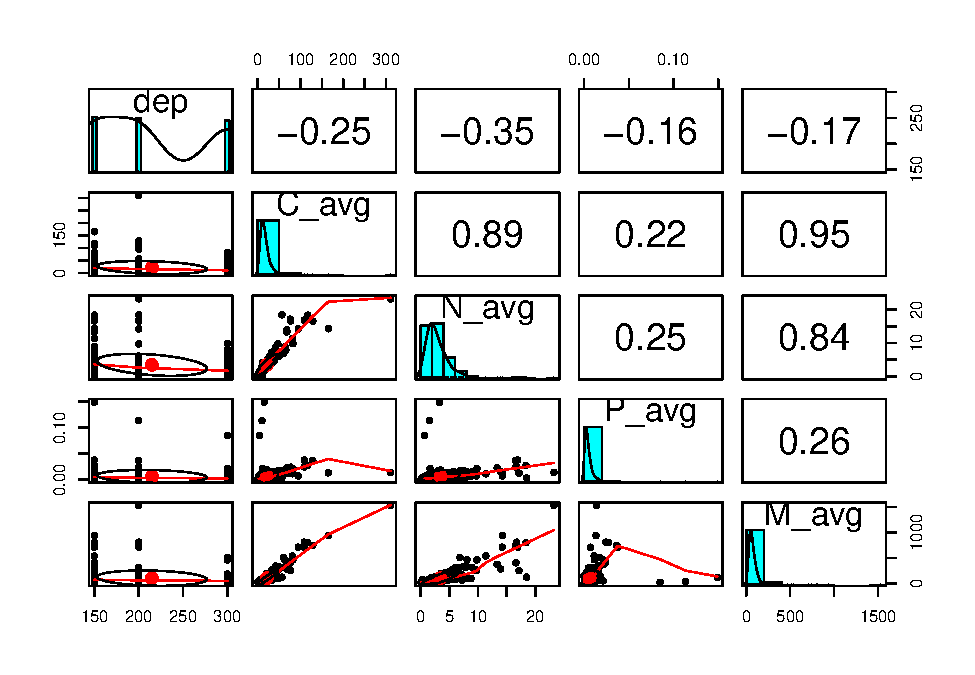
\includegraphics{Term_Project_files/figure-latex/unnamed-chunk-2-1.pdf}

\begin{Shaded}
\begin{Highlighting}[]
\KeywordTok{xyplot}\NormalTok{(M_avg }\OperatorTok{~}\StringTok{ }\NormalTok{C_avg }\OperatorTok{|}\StringTok{ }\NormalTok{dep, }
                  \DataTypeTok{main=}\StringTok{"Fig2a: Activity level-specific scatterplots"}
\NormalTok{           )}
\end{Highlighting}
\end{Shaded}

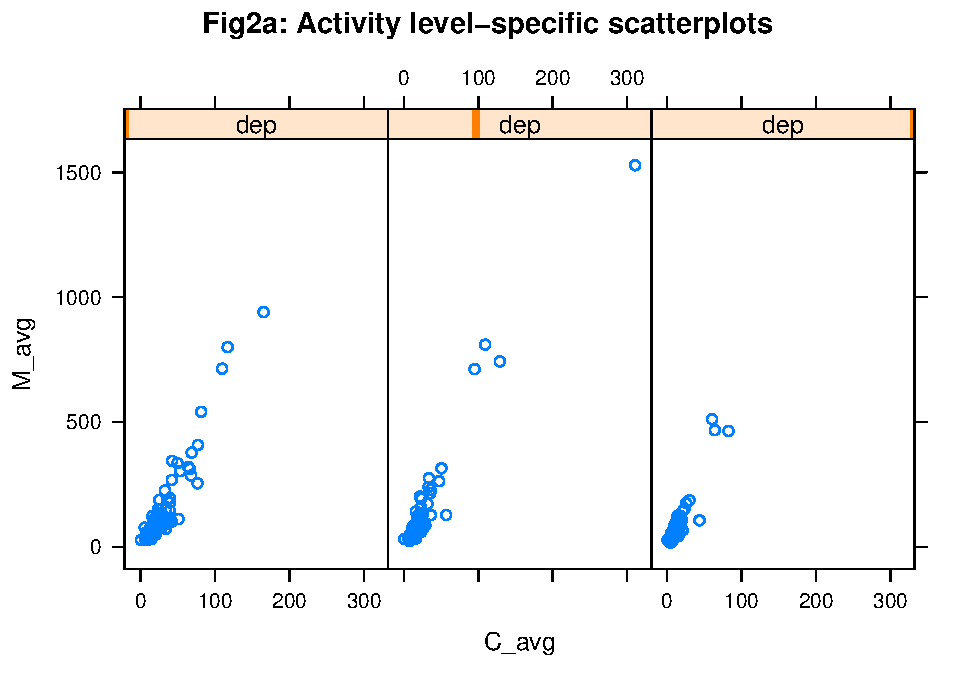
\includegraphics{Term_Project_files/figure-latex/unnamed-chunk-2-2.pdf}

\begin{Shaded}
\begin{Highlighting}[]
    \KeywordTok{xyplot}\NormalTok{(M_avg }\OperatorTok{~}\StringTok{ }\NormalTok{C_avg, }\DataTypeTok{groups=}\NormalTok{dep, }
                  \DataTypeTok{auto.key=}\OtherTok{TRUE}\NormalTok{,}
                  \DataTypeTok{main=}\StringTok{"Fig2b: Scatterplot with color=group level"}
\NormalTok{           )}
\end{Highlighting}
\end{Shaded}

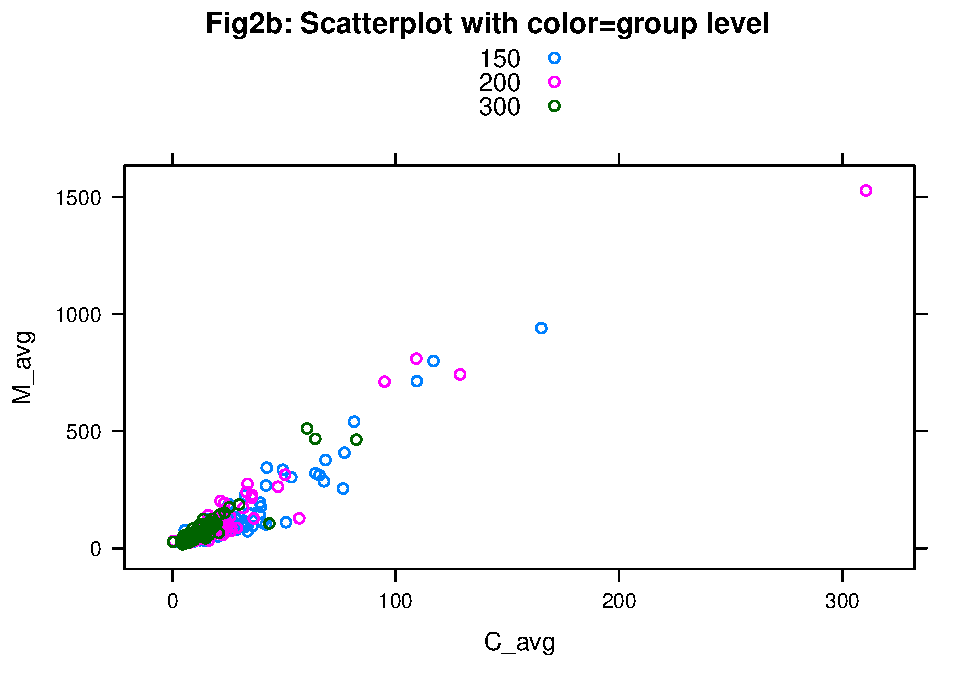
\includegraphics{Term_Project_files/figure-latex/unnamed-chunk-2-3.pdf}

\begin{Shaded}
\begin{Highlighting}[]
    \KeywordTok{xyplot}\NormalTok{(M_avg }\OperatorTok{~}\StringTok{ }\NormalTok{C_avg, }\DataTypeTok{groups=}\NormalTok{dep, }
                  \DataTypeTok{type=}\KeywordTok{c}\NormalTok{(}\StringTok{"p"}\NormalTok{,}\StringTok{"r"}\NormalTok{), }\CommentTok{# `p` for _points_, `r` for _regression line_}
                                   \CommentTok{# see https://stackoverflow.com/questions/12972039/plotting-xyplot-with-regression-line-on-lattice-graphics for more}
                  \DataTypeTok{auto.key=}\OtherTok{TRUE}\NormalTok{,}
                  \DataTypeTok{main=}\StringTok{"Fig3: Three standalone depth level-specific `lm()` fits"}
\NormalTok{           )}
\end{Highlighting}
\end{Shaded}

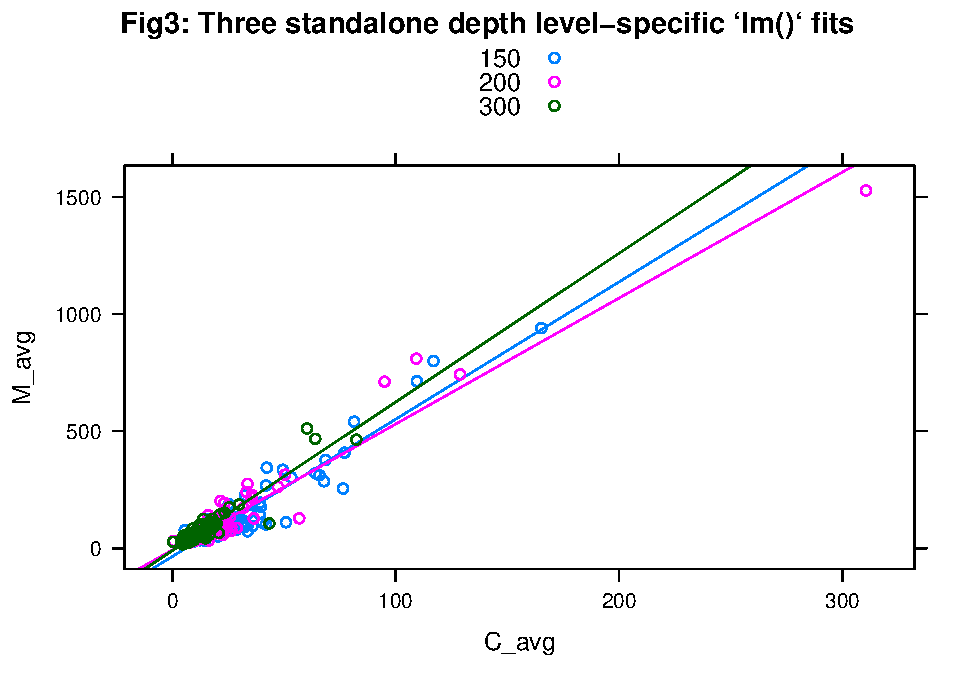
\includegraphics{Term_Project_files/figure-latex/unnamed-chunk-2-4.pdf}

Bar graph trial

\begin{Shaded}
\begin{Highlighting}[]
\CommentTok{# this code is to specify the depth I want to look at that contains the rows and the columns}
\NormalTok{Study_depths <-}\StringTok{ }\KeywordTok{c}\NormalTok{(}\StringTok{"150"}\NormalTok{, }\StringTok{"200"}\NormalTok{, }\StringTok{"300"}\NormalTok{, }\StringTok{"400"}\NormalTok{ ) }\CommentTok{#vector of depths I want to retain}

\NormalTok{Study_Rows <-}\StringTok{ }\KeywordTok{which}\NormalTok{(bats_flux}\OperatorTok{$}\NormalTok{dep }\OperatorTok\StringTok{ }\NormalTok{Study_depths) }\CommentTok{#which() to ask R which rows in spp name are on the list}


\NormalTok{bats_flux2 <-}\StringTok{ }\NormalTok{bats_flux[Study_Rows,] }\CommentTok{#has all the rows we want as well as all the columns}
\end{Highlighting}
\end{Shaded}

Mean and se of each depth of C-flux

\begin{Shaded}
\begin{Highlighting}[]
\NormalTok{Cflux <-}\StringTok{ }\NormalTok{bats_flux2[}\OperatorTok{-}\KeywordTok{which}\NormalTok{(}\KeywordTok{is.na}\NormalTok{(bats_flux2}\OperatorTok{$}\NormalTok{C_avg)),] }\CommentTok{#removes na from C-avg}
\NormalTok{Cflux.noNAs <-}\StringTok{ }\KeywordTok{delete.na}\NormalTok{(bats_flux2)}

\KeywordTok{levels}\NormalTok{(}\KeywordTok{as.factor}\NormalTok{(Cflux.noNAs}\OperatorTok{$}\NormalTok{dep150)) }\CommentTok{#this looks at the distribution of toxins in the organism selected}
\end{Highlighting}
\end{Shaded}

\begin{verbatim}
## character(0)
\end{verbatim}

\begin{Shaded}
\begin{Highlighting}[]
\NormalTok{dep150 <-}\StringTok{ }\KeywordTok{subset}\NormalTok{(Cflux.noNAs, dep}\OperatorTok{==}\StringTok{"150"}\NormalTok{) }\CommentTok{#focusing on mean of C-avg at depth 150}
\NormalTok{dep150}
\end{Highlighting}
\end{Shaded}

\begin{verbatim}
##        cr dep  yymmdd1  yymmdd2    decy1    decy2   Lat2 Lat2.1  Long1  Long2
## 710 10240 150 20081007 20081010 2008.766 2008.775 31.591 31.793 64.188 64.519
## 713 10241 150 20081108 20081111 2008.854 2008.863 31.577 31.361 64.184 64.051
## 719 10243 150 20090208 20090210 2009.104 2009.110 31.570 31.376 64.173 64.365
## 728 10246 150 20090515 20090518 2009.368 2009.376 31.582 31.700 64.162 64.309
## 731 10247 150 20090610 20090612 2009.439 2009.447 31.576 31.666 64.175 64.358
## 734 10248 150 20090714 20090716 2009.532 2009.540 31.566 31.348 64.166 64.191
## 737 10249 150 20090813 20090816 2009.616 2009.624 31.581 31.566 64.168 64.866
## 740 10250 150 20090910 20090913 2009.692 2009.700 31.576 31.309 64.169 63.801
## 746 10252 150 20091106 20091109 2009.849 2009.857 31.589 31.788 64.171 64.050
## 749 10253 150 20091208 20091210 2009.935 2009.941 31.595 31.103 64.154 63.851
## 767 10258 150 20100513 20100515 2010.362 2010.370 31.572 31.258 64.172 64.266
## 773 10260 150 20100722 20100726 2010.556 2010.565 31.578 31.583 64.183 64.352
## 782 10263 150 20101005 20101008 2010.761 2010.769 31.589 31.678 64.143 63.445
## 785 10264 150 20101109 20101112 2010.857 2010.864 31.583 31.833 64.177 64.016
## 788 10265 150 20101209 20101211 2010.937 2010.943 31.666 31.909 64.176 64.101
## 794 10267 150 20110325 20110328 2011.230 2011.238 31.593 31.576 64.185 64.746
## 800 10268 150 20110428 20110502 2011.322 2011.333 31.670 31.739 64.159 64.596
## 803 10269 150 20110517 20110520 2011.373 2011.381 31.581 31.672 64.158 63.963
## 815 10273 150 20110912 20110914 2011.698 2011.702 31.667 31.757 64.166 64.410
## 818 10274 150 20111102 20111105 2011.837 2011.844 31.668 31.652 64.186 65.038
## 821 10275 150 20111117 20111120 2011.877 2011.885 31.583 31.466 64.167 64.918
## 824 10276 150 20111207 20111210 2011.934 2011.942 31.581 31.806 64.174 64.540
## 827 10277 150 20120129 20120201 2012.077 2012.085 31.670 31.481 64.175 63.713
## 830 10278 150 20120210 20120211 2012.109 2012.112 31.664 31.597 64.167 64.018
## 833 10280 150 20120411 20120414 2012.276 2012.284 31.667 31.566 64.166 63.884
## 836 10281 150 20120518 20120522 2012.380 2012.390 31.751 31.823 64.167 65.222
## 839 10282 150 20120618 20120620 2012.462 2012.469 31.588 31.069 64.109 63.656
## 842 10283 150 20120712 20120715 2012.529 2012.537 31.612 30.979 64.202 64.292
## 851 10286 150 20121019 20121022 2012.798 2012.807 31.663 31.783 64.171 64.822
## 857 10288 150 20121210 20121213 2012.942 2012.950 31.668 31.387 64.165 63.495
## 860 10289 150 20130122 20130124 2013.059 2013.064 31.667 31.821 64.161 63.815
## 866 10291 150 20130312 20130314 2013.193 2013.200 31.662 31.179 64.168 64.553
## 869 10292 150 20130405 20130408 2013.260 2013.268 31.663 31.702 64.169 64.465
## 872 10293 150 20130515 20130517 2013.369 2013.374 31.672 31.614 64.171 64.274
## 878 10295 150 20130705 20130708 2013.509 2013.517 31.746 31.670 64.152 64.247
## 893 10300 150 20131209 20131211 2013.938 2013.945 31.671 31.715 64.200 64.234
## 896 10301 150 20140305 20140307 2014.173 2014.179 31.612 31.817 64.188 64.729
## 908 10305 150 20140709 20140712 2014.520 2014.528 31.657 31.511 64.169 64.396
## 911 10306 150 20140819 20140823 2014.633 2014.641 31.655 31.626 64.164 64.066
## 914 10307 150 20140913 20140916 2014.700 2014.708 31.663 31.579 64.166 64.382
## 917 10308 150 20141028 20141031 2014.823 2014.830 31.673 32.143 64.160 63.928
## 920 10309 150 20141119 20141122 2014.884 2014.893 31.670 31.641 64.163 63.971
## 923 10310 150 20141210 20141213 2014.940 2014.948 31.665 31.607 64.168 64.160
## 929 10312 150 20150312 20150315 2015.193 2015.200 31.640 31.456 64.125 64.094
## 932 10313 150 20150407 20150410 2015.265 2015.274 31.662 31.630 64.160 64.259
## 941 10316 150 20150715 20150718 2015.536 2015.543 31.654 31.424 64.159 64.222
## 944 10317 150 20150818 20150822 2015.629 2015.640 31.668 31.481 64.170 63.695
## 947 10318 150 20150912 20150914 2015.696 2015.704 31.661 31.587 64.163 63.880
##         M1      M2     M3  M_avg     C1     C2     C3  C_avg    N1    N2    N3
## 710  87.84   64.52 112.71  88.36  20.55  15.17  31.67  22.46  3.39  3.01  7.25
## 713 263.32   52.00  52.83 122.72  27.00  15.90   4.70  15.87  5.70  3.16  1.02
## 719 157.60   91.24  97.17 115.34  31.49  19.11  26.76  25.79  5.41  3.39  5.36
## 728  43.81   42.93  63.96  50.23  18.04  17.51  26.01  20.52  3.32  3.51  4.85
## 731  58.15  112.77  62.55  77.82  19.21  45.53  20.69  28.48  4.02 10.13  4.16
## 734  78.62  141.51  97.12 105.75  26.25  39.18  32.30  32.58  3.46  5.13  4.49
## 737  83.92  133.17 129.52 115.54  25.02  39.48  32.09  32.20  3.86  6.93  3.94
## 740  85.67  105.57 106.43  99.22  29.53  36.48  35.59  33.87  5.20  7.13  6.58
## 746  47.83   66.96  51.31  55.37  13.83  21.60  15.05  16.83  2.08  4.05  2.50
## 749  89.62  131.79  91.73 104.38  16.11  22.18  14.60  17.63  2.99  4.46  2.57
## 767  57.61   88.70  75.89  74.07  14.07  21.57  16.76  17.47  2.58  3.39  3.00
## 773  67.60   43.46  29.78  46.95  17.58  14.06   8.96  13.53  3.07  2.02  1.37
## 782  64.23   66.98  96.35  75.85  16.01  11.07  15.57  14.22  1.55  1.67  2.42
## 785  30.08   39.79  54.34  41.40   9.50  12.90  18.32  13.57  1.92  2.49  3.42
## 788 137.67  133.77 138.96 136.80  22.01  22.53  23.11  22.55  3.50  3.40  3.70
## 794 740.66  863.40 795.68 799.91 114.41 117.59 118.97 116.99 17.28 19.53 18.28
## 800  52.62   74.29  60.05  62.32  10.34  20.10  13.44  14.63  1.79  3.72  2.36
## 803  60.57  128.82 145.03 111.47  11.34  21.43  23.69  18.82  2.15  3.98  3.92
## 815 487.60  594.32 540.14 540.69  75.79  83.30  85.14  81.41  9.75 12.68 11.66
## 818  48.09   56.75  76.94  60.59  12.94  15.77  20.12  16.28  1.78  2.59  3.45
## 821  65.22   49.98  49.98  55.06  12.77   9.39  14.59  12.25  2.16  1.51  2.73
## 824 102.80   75.70  53.27  77.26  24.33  16.47  11.00  17.27  3.05  2.71  1.71
## 827 173.86  193.18 196.54 187.86  24.35  26.09  25.33  25.26  4.78  5.14  4.67
## 830 188.61  109.82 102.66 133.70  40.72  21.47  22.10  28.10  7.99  4.39  4.61
## 833 310.45  325.23 325.23 320.30  71.82  63.38  57.04  64.08  9.87  8.95  7.95
## 836  27.21   61.91  71.44  53.52   4.36  12.18  17.18  11.24  0.74  2.29  3.34
## 839  58.67  184.96  44.75  96.13  10.51  34.48  11.02  18.67  1.67  3.35  1.84
## 842 174.62  103.14 122.14 133.30  28.62  21.80  20.50  23.64  6.15  3.44  3.21
## 851  34.98   23.06  23.85  27.30   0.88   0.49   0.41   0.59  0.17  0.09  0.06
## 857  21.92   61.19  99.55  60.89   3.89  11.27  16.81  10.65  0.89  2.24  3.17
## 860 203.85  300.00 173.08 225.64  32.92  44.16  20.81  32.63  5.63  5.65  3.44
## 866 659.26  849.52 631.49 713.42 104.33 122.71 101.49 109.51 14.62 20.57 15.59
## 869 299.87  243.37 489.35 344.20  43.64  37.71  45.54  42.30  8.44  7.37  7.94
## 872  50.27   47.94  26.89  41.70  13.07  11.87   6.16  10.37  2.75  2.58  1.21
## 878  57.61   42.74  61.32  53.89  19.19  10.23  14.02  14.48  3.15  1.73  2.54
## 893  20.73   19.75  49.36  29.95   6.11   5.04  14.81   8.65  1.22  0.98  2.58
## 896  99.57  151.15 119.96 123.56  27.78  27.50  29.77  28.35  5.12  4.21  5.24
## 908 109.64   71.65 117.41  99.57  27.70  20.27  29.20  25.73  4.40  3.44  4.46
## 911 134.03   89.35 110.03 111.14  42.97  57.71  52.04  50.91  6.18  8.28  8.10
## 914  78.10   54.67  77.23  70.00  17.12  12.32  18.21  15.88  3.57  2.48  3.28
## 917  43.97   42.97  40.97  42.64  13.02  13.26  11.19  12.49  2.63  3.36  2.44
## 920  47.15   81.68  46.31  58.38  14.16  23.27  15.69  17.71  3.08  5.63  3.94
## 923  47.00   79.54  54.23  60.26  14.30  16.17  17.87  16.11  2.52  2.46  2.79
## 929 736.03 1109.13 974.93 940.03 132.67 191.04 171.97 165.23 11.69 16.29 14.90
## 932 277.95  325.81 306.50 303.42  50.59  52.22  56.99  53.27  6.42  6.45  7.39
## 941  97.35   71.06  77.88  82.10  25.62  18.29  20.56  21.49  4.07  2.36  3.07
## 944  97.33   99.22  96.70  97.75  26.81  25.73  26.57  26.37  3.51  2.99  3.48
## 947  68.34   77.24  90.51  78.70  20.36  22.17  26.93  23.15  2.64  2.64  3.88
##     N_avg     P1     P2     P3  P_avg   FBC1   FBC2   FBC3 FBC_avg  FBN1  FBN2
## 710  4.55 0.0071 0.0094 0.0160 0.0108  26.13  21.37  37.86   28.45  4.33  4.25
## 713  3.29 0.1419 0.1455 0.1593 0.1489  28.58  19.77   5.89   18.08  6.08  3.94
## 719  4.72 0.0061 0.0051 0.0054 0.0055  31.68  19.30  26.96   25.98  5.54  3.61
## 728  3.89 0.0063 0.0052 0.0060 0.0058  18.32  17.76  26.34   20.81  3.53  3.69
## 731  6.10 0.0091 0.0080 0.0095 0.0089  19.45  45.97  20.94   28.79  4.06 10.19
## 734  4.36 0.0128 0.0123 0.0128 0.0126  26.55  39.59  32.65   32.93  3.50  5.18
## 737  4.91 0.0061 0.0077 0.0114 0.0084  25.19  39.67  32.29   32.38  3.96  7.01
## 740  6.30 0.0125 0.0110 0.0089 0.0108  29.59  36.57  35.67   33.94  5.31  7.24
## 746  2.88 0.0015 0.0018 0.0020 0.0018  13.96  21.74  15.18   16.96  2.14  4.12
## 749  3.34 0.0060 0.0039 0.0058 0.0052  16.25  22.32  14.74   17.77  3.02  4.49
## 767  2.99 0.0184 0.0170 0.0152 0.0169  14.40  21.90  17.07   17.79  2.90  3.69
## 773  2.15 0.0058 0.0061 0.0070 0.0063  11.80  21.78   9.17   14.25  1.93  3.93
## 782  1.88 0.0142 0.0116 0.0092 0.0117  16.01  11.07  15.57   14.22  1.55  1.67
## 785  2.61 0.0044 0.0082 0.0061 0.0062   9.49  12.88  18.29   13.55  1.92  2.49
## 788  3.53 0.0275 0.0127 0.0151 0.0184  18.47  19.32  19.58   19.12  3.27  3.19
## 794 18.36 0.0274 0.0287 0.0255 0.0272 114.81 118.01 119.41  117.41 17.44 19.68
## 800  2.62 0.0065 0.0090 0.0149 0.0101   9.03  18.89  12.00   13.31  1.74  3.67
## 803  3.35 0.0137 0.0150 0.0114 0.0134  11.47  21.65  23.91   19.01  2.26  4.15
## 815 11.36 0.0128 0.0090 0.0121 0.0113  72.57  80.09  82.70   78.45  9.35 12.28
## 818  2.61 0.0053 0.0103 0.0047 0.0068  11.99  15.35  19.74   15.69  1.63  2.53
## 821  2.13 0.0079 0.0079 0.0092 0.0083  13.00   9.55  14.86   12.47  2.31  1.62
## 824  2.49 0.0091 0.0093 0.0196 0.0127  20.75  13.95   8.60   14.43  3.22  2.85
## 827  4.86 0.0060 0.0069 0.0070 0.0066  23.02  24.68  23.97   23.89  4.12  4.44
## 830  5.66 0.0043 0.0064 0.0069 0.0059  37.26  18.93  19.60   25.26  6.35  2.90
## 833  8.92 0.0121 0.0139 0.0187 0.0149  70.78  62.37  55.97   63.04  9.69  8.78
## 836  2.12 0.0064 0.0046 0.0054 0.0055   4.20  11.64  16.66   10.83  0.69  2.12
## 839  2.29 0.0032 0.0035 0.0031 0.0033   9.99  34.14  10.53   18.22  1.37  3.16
## 842  4.27 0.0050 0.0049 0.0051 0.0050  27.15  19.96  19.24   22.12  5.94  3.17
## 851  0.11 0.0011 0.0011 0.0007 0.0010   0.66   0.35   0.26    0.42  0.13  0.06
## 857  2.10 0.0031 0.0014 0.0024 0.0023   3.02  10.53  15.69    9.75  0.56  1.95
## 860  4.91 0.0033 0.0042 0.0061 0.0045  32.22  43.13  20.26   31.87  5.31  5.17
## 866 16.93 0.0372 0.0372 0.0387 0.0377 103.71 122.11 100.88  108.90 14.39 20.35
## 869  7.91 0.0166 0.0177 0.0128 0.0157  43.12  37.16  45.01   41.76  8.24  7.17
## 872  2.18 0.0021 0.0018 0.0021 0.0020  12.32  10.94   5.35    9.54  2.44  2.20
## 878  2.47 0.0057 0.0036 0.0043 0.0045  18.51   9.85  13.44   13.93  2.91  1.59
## 893  1.60 0.0021 0.0017 0.0018 0.0019   4.59   4.19  13.42    7.40  0.76  0.73
## 896  4.86 0.0075 0.0075 0.0081 0.0077  25.64  25.48  27.40   26.17  4.80  3.90
## 908  4.10 0.0052 0.0042 0.0038 0.0044  27.48  20.05  28.96   25.50  4.07  3.12
## 911  7.52 0.0018 0.0027 0.0055 0.0033  41.68  56.06  50.71   49.48  5.67  7.63
## 914  3.11 0.0059 0.0029 0.0030 0.0039  16.79  12.07  17.94   15.60  2.90  1.97
## 917  2.81 0.0024 0.0016 0.0009 0.0016  12.56  12.67  10.82   12.02  2.04  2.60
## 920  4.22 0.0014 0.0022 0.0013 0.0016  12.37  20.29  13.60   15.42  2.15  4.09
## 923  2.59 0.0027 0.0021 0.0016 0.0021  11.13  14.14  15.78   13.68  1.72  1.94
## 929 14.29 0.0143 0.0144 0.0108 0.0132 131.76 190.10 171.10  164.32 11.52 16.12
## 932  6.76 0.0046 0.0044 0.0051 0.0047  49.84  51.50  56.30   52.55  6.10  6.14
## 941  3.17 0.0030 0.0013 0.0029 0.0024  23.66  15.82  18.77   19.42  3.84  2.07
## 944  3.33 0.0019 0.0009 0.0041 0.0023  25.31  23.53  24.52   24.45  3.32  2.71
## 947  3.05 0.0011 0.0022 0.0007 0.0014  18.14  19.76  24.12   20.67  2.45  2.43
##      FBN3 FBN_avg
## 710  8.69    5.76
## 713  1.29    3.77
## 719  5.51    4.89
## 728  5.04    4.09
## 731  4.21    6.15
## 734  4.54    4.41
## 737  4.04    5.00
## 740  6.69    6.41
## 746  2.56    2.94
## 749  2.60    3.37
## 767  3.28    3.29
## 773  1.63    2.50
## 782  2.42    1.88
## 785  3.41    2.61
## 788  3.47    3.31
## 794 18.43   18.52
## 800  2.30    2.57
## 803  4.09    3.50
## 815 11.36   11.00
## 818  3.39    2.52
## 821  2.91    2.28
## 824  1.79    2.62
## 827  4.00    4.19
## 830  3.16    4.14
## 833  7.76    8.74
## 836  3.17    1.99
## 839  1.56    2.03
## 842  3.02    4.04
## 851  0.04    0.08
## 857  2.73    1.75
## 860  3.18    4.55
## 866 15.37   16.70
## 869  7.74    7.72
## 872  0.88    1.84
## 878  2.33    2.28
## 893  2.16    1.22
## 896  4.88    4.53
## 908  4.11    3.77
## 911  7.57    6.96
## 914  2.73    2.53
## 917  1.97    2.20
## 920  2.87    3.04
## 923  2.26    1.97
## 929 14.74   14.13
## 932  7.10    6.45
## 941  2.86    2.92
## 944  3.22    3.08
## 947  3.64    2.84
\end{verbatim}

\begin{Shaded}
\begin{Highlighting}[]
\NormalTok{muCflux150 <-}\StringTok{ }\KeywordTok{mean}\NormalTok{(dep150}\OperatorTok{$}\NormalTok{C_avg, }\DataTypeTok{data=}\NormalTok{dep150)}
\NormalTok{muCflux150}
\end{Highlighting}
\end{Shaded}

\begin{verbatim}
## [1] 30.46
\end{verbatim}

\begin{Shaded}
\begin{Highlighting}[]
\NormalTok{s.e150 <-}\StringTok{ }\NormalTok{muCflux150 }\OperatorTok{*}\StringTok{ }\KeywordTok{sqrt}\NormalTok{(}\DecValTok{10}\NormalTok{)}


\NormalTok{dep200 <-}\StringTok{ }\KeywordTok{subset}\NormalTok{(Cflux.noNAs, dep}\OperatorTok{==}\StringTok{"200"}\NormalTok{) }\CommentTok{#focusing on mean of C-avg at depth 200}
\NormalTok{dep200}
\end{Highlighting}
\end{Shaded}

\begin{verbatim}
##        cr dep  yymmdd1  yymmdd2    decy1    decy2   Lat2 Lat2.1  Long1  Long2
## 720 10243 200 20090208 20090210 2009.104 2009.110 31.570 31.376 64.173 64.365
## 723 10244 200 20090317 20090320 2009.206 2009.214 31.578 31.676 64.193 64.269
## 726 10245 200 20090414 20090416 2009.285 2009.289 31.576 31.675 64.166 63.973
## 729 10246 200 20090515 20090518 2009.368 2009.376 31.582 31.700 64.162 64.309
## 738 10249 200 20090813 20090816 2009.616 2009.624 31.581 31.566 64.168 64.866
## 741 10250 200 20090910 20090913 2009.692 2009.700 31.576 31.309 64.169 63.801
## 747 10252 200 20091106 20091109 2009.849 2009.857 31.589 31.788 64.171 64.050
## 750 10253 200 20091208 20091210 2009.935 2009.941 31.595 31.103 64.154 63.851
## 768 10258 200 20100513 20100515 2010.362 2010.370 31.572 31.258 64.172 64.266
## 771 10259 200 20100621 20100625 2010.471 2010.480 31.580 31.833 64.174 64.671
## 774 10260 200 20100722 20100726 2010.556 2010.565 31.578 31.583 64.183 64.352
## 783 10263 200 20101005 20101008 2010.761 2010.769 31.589 31.678 64.143 63.445
## 786 10264 200 20101109 20101112 2010.857 2010.864 31.583 31.833 64.177 64.016
## 795 10267 200 20110325 20110328 2011.230 2011.238 31.593 31.576 64.185 64.746
## 801 10268 200 20110428 20110502 2011.322 2011.333 31.670 31.739 64.159 64.596
## 804 10269 200 20110517 20110520 2011.373 2011.381 31.581 31.672 64.158 63.963
## 807 10270 200 20110614 20110617 2011.452 2011.460 31.574 31.426 64.169 64.585
## 813 10272 200 20110817 20110821 2011.627 2011.637 31.580 31.188 64.202 64.447
## 816 10273 200 20110912 20110914 2011.698 2011.702 31.667 31.757 64.166 64.410
## 819 10274 200 20111102 20111105 2011.837 2011.844 31.668 31.652 64.186 65.038
## 822 10275 200 20111117 20111120 2011.877 2011.885 31.583 31.466 64.167 64.918
## 825 10276 200 20111207 20111210 2011.934 2011.942 31.581 31.806 64.174 64.540
## 828 10277 200 20120129 20120201 2012.077 2012.085 31.670 31.481 64.175 63.713
## 831 10278 200 20120210 20120211 2012.109 2012.112 31.664 31.597 64.167 64.018
## 834 10280 200 20120411 20120414 2012.276 2012.284 31.667 31.566 64.166 63.884
## 837 10281 200 20120518 20120522 2012.380 2012.390 31.751 31.823 64.167 65.222
## 840 10282 200 20120618 20120620 2012.462 2012.469 31.588 31.069 64.109 63.656
## 846 10284 200 20120820 20120823 2012.635 2012.642 31.668 31.858 64.171 64.483
## 849 10285 200 20120911 20120914 2012.697 2012.705 31.666 31.744 64.161 64.415
## 852 10286 200 20121019 20121022 2012.798 2012.807 31.663 31.783 64.171 64.822
## 858 10288 200 20121210 20121213 2012.942 2012.950 31.668 31.387 64.165 63.495
## 861 10289 200 20130122 20130124 2013.059 2013.064 31.667 31.821 64.161 63.815
## 864 10290 200 20130212 20130215 2013.115 2013.124 31.667 31.540 64.167 64.090
## 867 10291 200 20130312 20130314 2013.193 2013.200 31.662 31.179 64.168 64.553
## 873 10293 200 20130515 20130517 2013.369 2013.374 31.672 31.614 64.171 64.274
## 879 10295 200 20130705 20130708 2013.509 2013.517 31.746 31.670 64.152 64.247
## 882 10296 200 20130802 20130804 2013.584 2013.591 31.663 31.177 64.172 64.357
## 888 10298 200 20131019 20131022 2013.799 2013.807 31.669 31.309 64.165 64.606
## 894 10300 200 20131209 20131211 2013.938 2013.945 31.671 31.715 64.200 64.234
## 897 10301 200 20140305 20140307 2014.173 2014.179 31.612 31.817 64.188 64.729
## 900 10302 200 20140411 20140414 2014.275 2014.283 31.700 31.745 64.138 64.345
## 903 10303 200 20140429 20140501 2014.323 2014.330 31.670 31.715 64.174 64.234
## 909 10305 200 20140709 20140712 2014.520 2014.528 31.657 31.511 64.169 64.396
## 912 10306 200 20140819 20140823 2014.633 2014.641 31.655 31.626 64.164 64.066
## 915 10307 200 20140913 20140916 2014.700 2014.708 31.663 31.579 64.166 64.382
## 918 10308 200 20141028 20141031 2014.823 2014.830 31.673 32.143 64.160 63.928
## 921 10309 200 20141119 20141122 2014.884 2014.893 31.670 31.641 64.163 63.971
## 927 10311 200 20150202 20150205 2015.089 2015.097 31.673 31.551 64.173 64.587
## 930 10312 200 20150312 20150315 2015.193 2015.200 31.640 31.456 64.125 64.094
## 939 10315 200 20150623 20150626 2015.474 2015.482 31.665 31.619 64.170 64.123
## 942 10316 200 20150715 20150718 2015.536 2015.543 31.654 31.424 64.159 64.222
## 945 10317 200 20150818 20150822 2015.629 2015.640 31.668 31.481 64.170 63.695
## 948 10318 200 20150912 20150914 2015.696 2015.704 31.661 31.587 64.163 63.880
##         M1      M2      M3   M_avg     C1     C2     C3  C_avg    N1    N2
## 720  77.02   39.10   27.25   47.79  13.99   8.47   7.91  10.12  1.94  1.35
## 723 183.56  301.98  236.00  240.51  31.26  37.73  30.70  33.23  5.53  6.78
## 726 119.16   97.65   79.44   98.75  23.96  24.46  17.09  21.84  3.20  2.67
## 729  53.45   81.49   39.43   58.12  20.45  33.90  13.64  22.66  2.40  7.01
## 738 101.25   81.18   86.65   89.69  27.71  26.83  24.62  26.39  4.10  4.74
## 741  84.80  121.14   63.17   89.70  20.63  23.22  18.47  20.77  3.30  3.43
## 747  41.74   41.74   75.65   53.04   8.21   7.45  16.18  10.61  1.28  1.17
## 750  86.46  111.76   94.89   97.70  16.03  29.77  21.45  22.42  2.65  5.74
## 768  74.98   57.61  105.15   79.25  15.54  13.21  22.62  17.12  2.61  2.21
## 771  41.33   41.33   54.04   45.57   9.61  10.41  12.20  10.74  1.64  2.07
## 774  37.82   30.58   33.00   33.80  11.38   9.29  10.24  10.30  1.56  1.43
## 783  84.42  155.99   76.16  105.52  23.32  27.55  12.85  21.24  2.77  2.61
## 786  25.23    6.79   36.87   22.96   8.15   1.85  12.83   7.61  1.30  0.32
## 795 785.53  847.32  796.53  809.79 109.98 112.32 105.45 109.25 17.26 16.84
## 801  58.20   48.91   60.05   55.72  12.90   9.75  11.54  11.40  2.54  1.70
## 804 122.00  142.47  125.41  129.96  19.05  24.03  20.14  21.07  3.23  4.14
## 807  62.30   57.98   63.17   61.15  10.67  10.28  12.23  11.06  1.80  1.68
## 813  93.31   62.21   82.69   79.40  10.20  10.84  14.20  11.75  0.17  0.14
## 816 819.24  702.67  612.37  711.43 119.23  94.73  71.13  95.03 19.43 14.07
## 819  56.75   48.09   53.86   52.90  10.90  10.70  10.01  10.54  1.81  1.73
## 822  45.74   68.61   53.36   55.90   8.74  15.16  11.09  11.66  1.16  2.34
## 825  48.60   50.46   42.05   47.04   8.02   9.03   6.10   7.72  1.19  1.24
## 828 111.71  125.99  127.67  121.79  14.43  15.98  21.79  17.40  2.82  3.13
## 831 126.53   64.46  174.28  121.76  25.80  12.66  21.67  20.04  5.21  2.75
## 834 225.23  448.71  268.71  314.22  41.39  62.98  47.24  50.54  4.71  7.66
## 837 121.78   75.52   68.03   88.44  21.12  12.65  11.86  15.21  3.24  2.12
## 840  64.64  100.44   85.52   83.53  16.25  19.61  18.87  18.24  2.19  3.26
## 846  67.83   28.42   62.33   52.86  12.81   6.80  12.86  10.82  1.93  0.99
## 849  45.92   71.91   39.85   52.56  10.32  13.62   9.22  11.05  1.69  2.39
## 852  27.03   34.98   31.80   31.27   0.54   0.65   0.78   0.66  0.20  0.13
## 858  47.49   36.53   37.44   40.49   8.55   7.15   9.65   8.45  1.42  1.59
## 861 121.79  165.38  135.90  141.02  15.02  18.21  15.05  16.09  2.21  3.13
## 864 227.19  118.50  170.80  172.16  34.47  21.37  39.50  31.78  5.21  3.28
## 867 738.45  756.96  732.28  742.56 125.86 118.29 142.40 128.85 18.26 15.29
## 873  39.75   36.24   37.41   37.80   9.07   8.47   8.85   8.79  1.81  1.54
## 879  16.72   34.38   44.60   31.90   4.32  10.57   9.38   8.09  0.78  1.81
## 882  45.94   50.72   50.72   49.13  10.19  10.79   5.56   8.85  1.68  1.73
## 888  30.43   34.55   51.82   38.93   6.29   7.24  10.84   8.12  1.03  1.20
## 894  25.67   32.58   17.77   25.34   7.91   8.12   6.10   7.38  1.47  1.38
## 897 141.55  109.16  135.55  128.75  25.81  20.43  23.14  23.13  4.26  3.11
## 900 139.70  200.81  136.79  159.10  20.14  28.83  20.85  23.27  3.61  4.82
## 903  66.67   63.59   68.72   66.33  20.62  10.37  16.64  15.88  3.42  2.02
## 909  49.21   75.97   84.60   69.93  13.33  19.64  21.94  18.30  2.55  3.14
## 912  59.57  104.24   96.80   86.87  22.53  32.51  31.38  28.81  3.84  4.80
## 915  73.76   42.52   45.12   53.80  13.99   9.64   8.59  10.74  2.30  2.45
## 918  47.96   28.98   40.97   39.30  11.91   8.09   6.68   8.89  2.28  3.60
## 921  37.05   33.68   29.47   33.40  10.86   8.50  12.43  10.60  3.03  2.13
## 927 135.62  153.11  115.49  134.74  25.42  29.12  23.01  25.85  2.85  2.94
## 930 653.68 1973.25 1956.98 1527.97 252.04 410.30 269.56 310.63 19.12 30.63
## 939  82.83   49.53   48.67   60.34  11.25   7.27  18.98  12.50  1.96  1.19
## 942  85.66   90.53   90.53   88.91  18.06  21.26  20.45  19.92  2.33  2.35
## 945  48.98   64.05   74.73   62.59  11.73  14.16  18.21  14.70  1.39  1.39
## 948  64.61   70.57   86.68   73.95  15.04  15.66  16.21  15.64  1.53  1.46
##        N3 N_avg     P1     P2     P3  P_avg   FBC1   FBC2   FBC3 FBC_avg  FBN1
## 720  1.28  1.52 0.0049 0.0036 0.0039 0.0041  14.12   8.59   8.04   10.25  2.09
## 723  5.24  5.85 0.0146 0.0075 0.0065 0.0095  31.43  37.92  30.88   33.41  5.56
## 726  3.24  3.04 0.0011 0.0026 0.0039 0.0025  24.21  24.72  17.27   22.07  3.37
## 729  2.26  3.89 0.0038 0.0052 0.0043 0.0044  20.85  34.27  13.86   22.99  2.78
## 738  3.18  4.01 0.0189 0.0094 0.0028 0.0104  27.89  27.02  24.79   26.57  4.19
## 741  2.72  3.15 0.0057 0.0036 0.0097 0.0063  20.67  23.27  18.51   20.82  3.42
## 747  2.61  1.69 0.0025 0.0020 0.0026 0.0024   8.34   7.61  16.33   10.76  1.33
## 750  3.27  3.89 0.0024 0.0028 0.0020 0.0024  16.19  29.93  21.61   22.58  2.68
## 768  4.31  3.04 0.0141 0.0199 0.0103 0.0148  15.88  13.58  22.99   17.48  2.92
## 771  2.32  2.01 0.0027 0.0037 0.0034 0.0033   9.96  10.67  12.57   11.07  2.12
## 774  1.40  1.46 0.0022 0.0025 0.0026 0.0024  11.62   9.49  10.53   10.55  1.86
## 783  1.89  2.42 0.0032 0.0106 0.0117 0.0085  23.33  27.55  12.85   21.24  2.77
## 786  1.14  0.92 0.0034 0.0042 0.0028 0.0035   8.14   1.85  12.82    7.60  1.30
## 795 16.13 16.74 0.0171 0.0250 0.0315 0.0245 110.40 112.71 105.85  109.65 17.42
## 801  2.02  2.09 0.0057 0.0060 0.0031 0.0049  11.56   8.16  10.03    9.92  2.48
## 804  2.98  3.45 0.0129 0.0062 0.0105 0.0099  19.29  24.29  20.40   21.33  3.43
## 807  1.53  1.67 0.0115 0.0020 0.0030 0.0055  11.14  10.77  12.62   11.51  2.11
## 813  0.71  0.34 0.0046 0.0045 0.0050 0.0047  10.14  10.75  14.16   11.68  1.42
## 816  9.25 14.25 0.0069 0.0068 0.0075 0.0071 114.03  90.37  67.56   90.65 18.80
## 819  1.67  1.74 0.0029 0.0025 0.0024 0.0026  10.48  10.31   9.59   10.13  1.74
## 822  1.44  1.65 0.0535 0.0053 0.0050 0.0213   8.90  15.43  11.29   11.87  1.25
## 825  0.84  1.09 0.0070 0.0100 0.0058 0.0076   5.74   5.24   4.09    5.02  1.25
## 828  4.60  3.52 0.0034 0.0029 0.0042 0.0035  13.02  14.57  20.34   15.98  2.12
## 831  4.64  4.20 0.0043 0.0047 0.0046 0.0045  22.40  10.90  19.10   17.47  3.12
## 834  5.88  6.08 0.0077 0.0088 0.0085 0.0083  40.36  61.57  46.06   49.33  4.52
## 837  1.70  2.35 0.0071 0.0036 0.0040 0.0049  20.46  12.03  11.32   14.60  3.04
## 840  2.95  2.80 0.0016 0.0019 0.0013 0.0016  15.31  18.49  17.22   17.01  1.64
## 846  1.72  1.55 0.0021 0.0014 0.0017 0.0017  11.86   5.52  11.67    9.68  1.76
## 849  1.27  1.79 0.0018 0.0008 0.0008 0.0011   9.51  12.62   8.32   10.15  1.39
## 852  0.12  0.15 0.0007 0.0004 0.0009 0.0007   0.37   0.44   0.59    0.47  0.17
## 858  1.22  1.41 0.0017 0.0030 0.0014 0.0020   7.75   5.86   8.63    7.41  1.11
## 861  2.25  2.53 0.0014 0.0042 0.0037 0.0031  14.29  17.47  14.36   15.37  1.87
## 864  4.47  4.32 0.0151 0.0141 0.0115 0.0136  33.83  20.89  38.86   31.19  4.95
## 867 16.17 16.57 0.0361 0.0351 0.0382 0.0365 125.26 117.67 141.80  128.24 18.04
## 873  1.70  1.68 0.0014 0.0039 0.0010 0.0021   8.25   7.87   8.12    8.08  1.48
## 879  2.23  1.61 0.0025 0.0029 0.0030 0.0028   4.10   9.95   8.94    7.66  0.70
## 882  1.75  1.72 0.0041 0.0025 0.0050 0.0039   9.52  10.18   4.96    8.22  1.54
## 888  2.29  1.51 0.0015 0.0026 0.0024 0.0022   5.27   6.00   8.38    6.55  0.85
## 894  1.07  1.31 0.0013 0.0002 0.0005 0.0007   5.53   6.51   4.80    5.61  0.75
## 897  3.99  3.79 0.0058 0.0029 0.0041 0.0043  23.82  18.58  21.28   21.23  3.96
## 900  3.87  4.10 0.0056 0.0045 0.0051 0.0051  17.60  26.11  18.34   20.68  2.87
## 903  3.41  2.95 0.0020 0.0029 0.0017 0.0022  18.56   9.08  14.46   14.03  2.53
## 909  3.71  3.14 0.0031 0.0024 0.0034 0.0030  13.08  19.37  21.69   18.05  2.18
## 912  5.33  4.66 0.0015 0.0012 0.0025 0.0017  21.09  30.91  29.83   27.28  3.27
## 915  1.87  2.21 0.0015 0.0017 0.0015 0.0016  13.63   9.15   8.29   10.36  1.56
## 918  1.60  2.49 0.0011 0.0019 0.0006 0.0012  11.54   6.80   6.24    8.19  1.80
## 921  2.41  2.52 0.0007 0.0003 0.0009 0.0006   8.54   6.84   9.80    8.39  1.83
## 927  2.58  2.79 0.0030 0.0032 0.0025 0.0029  24.70  28.48  22.29   25.16  2.54
## 930 20.03 23.26 0.0154 0.0145 0.0116 0.0138 251.11 409.05 268.56  309.57 18.95
## 939  2.46  1.87 0.0011 0.0029 0.0018 0.0019   9.71   5.86  16.71   10.76  1.62
## 942  2.63  2.44 0.0020 0.0016 0.0005 0.0014  16.16  19.33  18.81   18.10  2.11
## 945  2.33  1.71 0.0023 0.0027 0.0009 0.0020   9.53  12.56  16.59   12.89  1.11
## 948  1.80  1.60 0.0005 0.0008 0.0008 0.0007  13.15  13.82  12.68   13.22  1.37
##      FBN2  FBN3 FBN_avg
## 720  1.51  1.46    1.69
## 723  6.81  5.27    5.88
## 726  2.87  3.37    3.20
## 729  7.18  2.44    4.13
## 738  4.84  3.28    4.10
## 741  3.53  2.83    3.26
## 747  1.24  2.67    1.75
## 750  5.79  3.31    3.93
## 768  2.57  4.64    3.38
## 771  2.41  2.81    2.45
## 774  1.69  1.79    1.78
## 783  2.61  1.89    2.42
## 786  0.32  1.14    0.92
## 795 17.00 16.29   16.90
## 801  1.64  1.96    2.03
## 804  4.35  3.19    3.66
## 807  2.00  1.77    1.96
## 813  1.58  2.04    1.68
## 816 13.53  8.80   13.71
## 819  1.67  1.61    1.67
## 822  2.50  1.54    1.76
## 825  1.29  0.88    1.14
## 828  2.43  3.88    2.81
## 831  1.63  3.12    2.62
## 834  7.41  5.67    5.87
## 837  1.93  1.53    2.17
## 840  2.61  1.99    2.08
## 846  0.76  1.51    1.34
## 849  2.02  0.94    1.45
## 852  0.08  0.08    0.11
## 858  1.08  0.82    1.00
## 861  2.79  1.93    2.20
## 864  3.09  4.22    4.09
## 867 15.06 15.95   16.35
## 873  1.30  1.42    1.40
## 879  1.59  2.07    1.45
## 882  1.60  1.62    1.59
## 888  0.98  1.84    1.22
## 894  0.89  0.68    0.77
## 897  2.83  3.71    3.50
## 900  4.03  3.14    3.35
## 903  1.47  2.47    2.16
## 909  2.76  3.35    2.76
## 912  4.16  4.72    4.05
## 915  1.45  1.25    1.42
## 918  1.95  1.04    1.60
## 921  1.28  1.06    1.39
## 927  2.66  2.26    2.49
## 930 30.40 19.84   23.06
## 939  0.88  1.96    1.49
## 942  2.12  2.44    2.22
## 945  1.19  2.13    1.48
## 948  1.31  1.50    1.39
\end{verbatim}

\begin{Shaded}
\begin{Highlighting}[]
\NormalTok{muCflux200 <-}\StringTok{ }\KeywordTok{mean}\NormalTok{(dep200}\OperatorTok{$}\NormalTok{C_avg, }\DataTypeTok{data=}\NormalTok{dep200)}
\NormalTok{muCflux200}
\end{Highlighting}
\end{Shaded}

\begin{verbatim}
## [1] 27.05189
\end{verbatim}

\begin{Shaded}
\begin{Highlighting}[]
\NormalTok{dep300 <-}\StringTok{ }\KeywordTok{subset}\NormalTok{(Cflux.noNAs, dep}\OperatorTok{==}\StringTok{"300"}\NormalTok{) }\CommentTok{#focusing on mean of C-avg at depth 300}
\NormalTok{dep300}
\end{Highlighting}
\end{Shaded}

\begin{verbatim}
##        cr dep  yymmdd1  yymmdd2    decy1    decy2   Lat2 Lat2.1  Long1  Long2
## 715 10241 300 20081108 20081111 2008.854 2008.863 31.577 31.361 64.184 64.051
## 724 10244 300 20090317 20090320 2009.206 2009.214 31.578 31.676 64.193 64.269
## 727 10245 300 20090414 20090416 2009.285 2009.289 31.576 31.675 64.166 63.973
## 730 10246 300 20090515 20090518 2009.368 2009.376 31.582 31.700 64.162 64.309
## 733 10247 300 20090610 20090612 2009.439 2009.447 31.576 31.666 64.175 64.358
## 736 10248 300 20090714 20090716 2009.532 2009.540 31.566 31.348 64.166 64.191
## 739 10249 300 20090813 20090816 2009.616 2009.624 31.581 31.566 64.168 64.866
## 742 10250 300 20090910 20090913 2009.692 2009.700 31.576 31.309 64.169 63.801
## 745 10251 300 20091009 20091012 2009.771 2009.778 31.596 31.731 64.180 64.417
## 748 10252 300 20091106 20091109 2009.849 2009.857 31.589 31.788 64.171 64.050
## 769 10258 300 20100513 20100515 2010.362 2010.370 31.572 31.258 64.172 64.266
## 772 10259 300 20100621 20100625 2010.471 2010.480 31.580 31.833 64.174 64.671
## 787 10264 300 20101109 20101112 2010.857 2010.864 31.583 31.833 64.177 64.016
## 796 10267 300 20110325 20110328 2011.230 2011.238 31.593 31.576 64.185 64.746
## 802 10268 300 20110428 20110502 2011.322 2011.333 31.670 31.739 64.159 64.596
## 805 10269 300 20110517 20110520 2011.373 2011.381 31.581 31.672 64.158 63.963
## 808 10270 300 20110614 20110617 2011.452 2011.460 31.574 31.426 64.169 64.585
## 811 10271 300 20110705 20110709 2011.509 2011.518 31.583 32.182 64.171 64.075
## 817 10273 300 20110912 20110914 2011.698 2011.702 31.667 31.757 64.166 64.410
## 823 10275 300 20111117 20111120 2011.877 2011.885 31.583 31.466 64.167 64.918
## 826 10276 300 20111207 20111210 2011.934 2011.942 31.581 31.806 64.174 64.540
## 829 10277 300 20120129 20120201 2012.077 2012.085 31.670 31.481 64.175 63.713
## 832 10278 300 20120210 20120211 2012.109 2012.112 31.664 31.597 64.167 64.018
## 835 10280 300 20120411 20120414 2012.276 2012.284 31.667 31.566 64.166 63.884
## 838 10281 300 20120518 20120522 2012.380 2012.390 31.751 31.823 64.167 65.222
## 841 10282 300 20120618 20120620 2012.462 2012.469 31.588 31.069 64.109 63.656
## 847 10284 300 20120820 20120823 2012.635 2012.642 31.668 31.858 64.171 64.483
## 853 10286 300 20121019 20121022 2012.798 2012.807 31.663 31.783 64.171 64.822
## 856 10287 300 20121114 20121117 2012.871 2012.879 31.665 31.440 64.163 64.650
## 859 10288 300 20121210 20121213 2012.942 2012.950 31.668 31.387 64.165 63.495
## 862 10289 300 20130122 20130124 2013.059 2013.064 31.667 31.821 64.161 63.815
## 865 10290 300 20130212 20130215 2013.115 2013.124 31.667 31.540 64.167 64.090
## 868 10291 300 20130312 20130314 2013.193 2013.200 31.662 31.179 64.168 64.553
## 874 10293 300 20130515 20130517 2013.369 2013.374 31.672 31.614 64.171 64.274
## 880 10295 300 20130705 20130708 2013.509 2013.517 31.746 31.670 64.152 64.247
## 898 10301 300 20140305 20140307 2014.173 2014.179 31.612 31.817 64.188 64.729
## 901 10302 300 20140411 20140414 2014.275 2014.283 31.700 31.745 64.138 64.345
## 910 10305 300 20140709 20140712 2014.520 2014.528 31.657 31.511 64.169 64.396
## 916 10307 300 20140913 20140916 2014.700 2014.708 31.663 31.579 64.166 64.382
## 919 10308 300 20141028 20141031 2014.823 2014.830 31.673 32.143 64.160 63.928
## 922 10309 300 20141119 20141122 2014.884 2014.893 31.670 31.641 64.163 63.971
## 925 10310 300 20141210 20141213 2014.940 2014.948 31.665 31.607 64.168 64.160
## 928 10311 300 20150202 20150205 2015.089 2015.097 31.673 31.551 64.173 64.587
## 943 10316 300 20150715 20150718 2015.536 2015.543 31.654 31.424 64.159 64.222
## 946 10317 300 20150818 20150822 2015.629 2015.640 31.668 31.481 64.170 63.695
##         M1     M2     M3  M_avg    C1    C2     C3 C_avg   N1   N2    N3 N_avg
## 715  25.59  34.67  18.99  26.42  5.06  6.97   3.06  5.03 0.62 1.08  0.41  0.70
## 724 176.79 146.34 202.17 175.10 24.96 21.35  30.43 25.58 5.05 3.71  5.26  4.67
## 727  29.79  87.72  26.48  48.00  8.93 14.63   6.66 10.07 1.58 2.00  0.48  1.35
## 730  38.55  85.87  28.04  50.82 14.45 15.90   8.72 13.02 2.02 2.86  1.24  2.04
## 733  32.60  20.26  32.60  28.49  7.46  4.42   8.09  6.66 1.30 0.71  1.47  1.16
## 736  62.90  49.95  61.97  58.27 14.65 11.51  19.33 15.16 2.20 1.71  3.61  2.51
## 739  58.38  52.90  58.38  56.55 15.90 16.15  17.47 16.51 2.52 2.72  2.92  2.72
## 742 101.24  84.80  91.72  92.59 17.85 13.70  24.92 18.82 2.56 1.64  2.26  2.15
## 745 162.62 245.27  47.99 151.96 45.69 15.17   9.39 23.42 9.15 2.75  1.30  4.40
## 748  60.00  58.26  68.70  62.32 11.56 16.77  10.90 13.08 1.60 1.11  1.45  1.39
## 769  48.46  25.60  20.12  31.39 13.18  6.04   5.38  8.20 1.81 1.04  0.64  1.16
## 772  38.94  48.48  38.15  41.86  7.75  8.13   3.17  6.35 1.09 1.37  0.50  0.99
## 787  47.55  24.26  30.08  33.96 11.31  0.12   2.44  4.62 1.68 0.05  0.31  0.68
## 796 444.40 545.13 402.07 463.87 67.79 71.94 107.44 82.39 9.54 9.84 10.08  9.82
## 802  67.48  69.34  60.67  65.83 10.67 11.33  10.76 10.92 1.82 1.96  1.82  1.87
## 805 106.64  98.96 112.61 106.07 29.75 13.15  16.49 19.80 4.56 2.11  2.53  3.07
## 808  63.17  43.27  49.32  51.92 10.83  7.97  11.46 10.09 2.08 1.25  1.56  1.63
## 811  42.35  63.14  50.05  51.85  7.36 10.64  10.77  9.59 0.95 1.52  1.35  1.27
## 817 438.35 446.56 517.15 467.35 54.75 64.18  73.11 64.01 6.66 7.78  9.84  8.09
## 823  40.66  48.28  44.89  44.61  6.73  8.57   7.80  7.70 0.95 2.29  1.29  1.51
## 826  56.07  47.66  57.94  53.89  7.62  6.03   7.40  7.02 1.04 0.77  0.86  0.89
## 829  88.19  73.07  90.71  83.99  9.13  8.10  10.05  9.09 1.91 1.61  1.98  1.83
## 832  95.50  93.11  71.62  86.74 17.21 15.19  12.68 15.03 3.64 3.28  2.92  3.28
## 835 194.79 159.14 206.10 186.68 32.09 30.46  27.33 29.96 3.72 3.63  3.04  3.46
## 838  58.51  39.46  65.99  54.65  8.33  4.58   8.75  7.22 1.23 0.92  1.03  1.06
## 841  26.85  31.82  61.65  40.11  7.17  6.50  13.91  9.19 1.28 1.13  1.48  1.29
## 847  46.75  43.08  42.17  44.00 10.20  8.26   7.08  8.52 1.37 0.98  0.94  1.10
## 853  32.60  31.80  18.29  27.56  0.28  0.55   0.40  0.41 0.07 0.07  0.06  0.07
## 856  26.43  26.43  25.61  26.16  1.55  4.93   5.07  3.85 0.55 1.06  1.06  0.89
## 859  48.40  57.54  29.22  45.05 11.07  6.84   6.86  8.26 1.46 1.24  0.88  1.20
## 862  39.74  48.72  67.95  52.14  4.46  4.94   5.78  5.06 0.76 0.82  0.93  0.84
## 865  63.75  68.81  51.49  61.35 13.04 18.18  11.00 14.08 1.92 2.47  1.64  2.01
## 868 519.38 497.78 516.30 511.15 52.57 46.19  82.26 60.34 6.84 6.49  7.23  6.85
## 874  42.09  28.06  35.08  35.08  7.89  5.39   7.16  6.81 1.38 0.99  1.31  1.23
## 880  19.51  35.31  43.67  32.83  4.90  5.83   6.54  5.76 0.87 0.74  1.69  1.10
## 898 137.95  89.97  75.57 101.16 23.25 13.48  15.10 17.28 2.66 1.95  2.23  2.28
## 901  59.18  78.58  52.39  63.38 10.50 13.97  12.24 12.24 1.86 3.39  3.32  2.86
## 910  46.62  61.29  31.94  46.62 10.94 15.86   7.01 11.27 1.70 2.23  1.00  1.64
## 916  64.21  95.45  98.92  86.19  9.31  8.13  19.10 12.18 1.66 2.10  3.55  2.44
## 919  31.98  31.98  40.97  34.98  8.09  6.08   7.43  7.20 2.00 1.62  1.62  1.75
## 922  18.52  34.52  37.89  30.31  5.99 10.53   9.68  8.74 1.65 2.60  3.71  2.65
## 925  33.44  42.48  37.96  37.96  9.86 10.73   6.81  9.14 2.24 1.94  1.19  1.79
## 928  92.74  69.12  78.74  80.20 19.37 14.98  15.30 16.55 2.16 1.55  1.75  1.82
## 943  78.85  91.51  80.80  83.72 18.23 18.30  17.12 17.88 2.56 1.76  1.79  2.04
## 946  62.79  77.24  77.24  72.42 13.20 16.27  15.91 15.13 1.47 1.63  1.63  1.58
##         P1     P2     P3  P_avg  FBC1  FBC2   FBC3 FBC_avg FBN1  FBN2  FBN3
## 715 0.0657 0.0859 0.1034 0.0850  8.49  9.85   6.62    8.32 1.08  1.55  0.91
## 724 0.0052 0.0056 0.0072 0.0060 25.12 21.50  30.61   25.74 5.08  3.74  5.29
## 727 0.0022 0.0021 0.0012 0.0018  9.36 14.83   6.94   10.38 2.05  2.17  0.79
## 730 0.0031 0.0021 0.0034 0.0029 14.72 16.13   8.99   13.28 2.27  3.02  1.55
## 733 0.0019 0.0014 0.0018 0.0017  7.72  4.52   8.30    6.85 1.38  0.74  1.53
## 736 0.0057 0.0042 0.0067 0.0055 14.86 11.71  19.58   15.38 2.24  1.76  3.66
## 739 0.0043 0.0029 0.0029 0.0034 16.05 16.30  17.63   16.66 2.62  2.82  3.02
## 742 0.0049 0.0028 0.0052 0.0043 17.87 13.72  24.97   18.85 2.67  1.75  2.36
## 745 0.0018 0.0021 0.0025 0.0021 46.08 15.41   9.50   23.66 9.24  2.82  1.33
## 748 0.0014 0.0012 0.0020 0.0015 11.73 16.95  11.05   13.24 1.67  1.16  1.51
## 769 0.0100 0.0072 0.0084 0.0085 13.55  6.34   6.89    8.93 2.18  1.34  2.22
## 772 0.0026 0.0021 0.0021 0.0023  7.99  8.43   3.29    6.57 1.41  1.78  0.66
## 787 0.0025 0.0017 0.0030 0.0024 11.29  0.12   2.43    4.61 1.68  0.05  0.31
## 796 0.0182 0.0219 0.0238 0.0213 68.11 72.26 107.90   82.76 9.72 10.01 10.26
## 802 0.0034 0.0048 0.0048 0.0043  9.46  9.92   9.52    9.63 1.77  1.90  1.77
## 805 0.0043 0.0048 0.0180 0.0090 30.26 13.39  16.76   20.14 4.97  2.31  2.75
## 808 0.0013 0.0021 0.0012 0.0015 11.26  8.42  11.98   10.55 2.36  1.54  1.89
## 811 0.0029 0.0044 0.0038 0.0037 26.03  6.11  10.57   14.24 2.92  0.85  1.58
## 817 0.0069 0.0238 0.0036 0.0114 50.53 58.97  66.88   58.79 6.13  7.11  9.04
## 823 0.0051 0.0048 0.0057 0.0052  6.85  8.72   7.94    7.84 1.03  2.45  1.38
## 826 0.0040 0.0058 0.0082 0.0060  5.08  3.54   4.54    4.39 1.09  0.80  0.89
## 829 0.0029 0.0033 0.0020 0.0027  7.54  6.55   8.72    7.60 1.12  0.85  1.32
## 832 0.0037 0.0033 0.0037 0.0036 14.93 13.17  10.52   12.87 2.23  2.02  1.45
## 835 0.0053 0.0068 0.0040 0.0054 30.89 29.26  26.32   28.82 3.51  3.42  2.86
## 838 0.0021 0.0020 0.0023 0.0021  7.66  3.69   8.10    6.48 1.02  0.64  0.83
## 841 0.0006 0.0009 0.0007 0.0007  6.06  5.70  13.31    8.36 0.63  0.67  1.13
## 847 0.0012 0.0007 0.0016 0.0012  9.00  7.15   6.19    7.45 1.16  0.79  0.79
## 853 0.0002 0.0005 0.0005 0.0004  0.08  0.36   0.29    0.24 0.03  0.03  0.04
## 856 0.0002 0.0004 0.0004 0.0003  0.91  4.23   4.52    3.22 0.19  0.67  0.75
## 859 0.0027 0.0017 0.0020 0.0021 10.00  6.08   5.64    7.24 1.05  0.95  0.41
## 862 0.0010 0.0017 0.0008 0.0012  3.69  4.01   5.15    4.28 0.40  0.39  0.64
## 865 0.0022 0.0036 0.0016 0.0025 12.26 17.34  10.02   13.21 1.62  2.13  1.26
## 868 0.0200 0.0195 0.0125 0.0173 51.95 45.59  81.65   59.73 6.61  6.27  7.01
## 874 0.0012 0.0005 0.0010 0.0009  6.76  4.84   6.21    5.94 0.93  0.77  0.94
## 880 0.0013 0.0010 0.0013 0.0012  4.48  5.37   5.87    5.24 0.72  0.58  1.45
## 898 0.0015 0.0021 0.0007 0.0014 21.34 11.25  12.51   15.03 2.37  1.61  1.84
## 901 0.0014 0.0019 0.0013 0.0015  7.68  7.97   6.97    7.54 1.03  1.63  1.77
## 910 0.0016 0.0024 0.0026 0.0022 10.67 15.63   6.85   11.05 1.31  1.91  0.77
## 916 0.0016 0.0010 0.0005 0.0010  8.96  7.65  18.62   11.74 0.96  1.12  2.59
## 919 0.0005 0.0008 0.0008 0.0007  7.53  5.67   6.82    6.67 1.29  1.10  0.85
## 922 0.0005 0.0004 0.0003 0.0004  4.14  7.98   4.18    5.43 0.70  1.28  0.88
## 925 0.0005 0.0004 0.0004 0.0004  5.66  6.72   3.62    5.33 1.18  0.92  0.38
## 928 0.0008 0.0016 0.0008 0.0011 18.46 14.10  14.27   15.61 1.76  1.17  1.31
## 943 0.0027 0.0017 0.0013 0.0019 15.96 16.37  14.80   15.71 2.29  1.53  1.51
## 946 0.0010 0.0016 0.0019 0.0015 11.50 14.56  14.41   13.49 1.25  1.41  1.44
##     FBN_avg
## 715    1.18
## 724    4.70
## 727    1.67
## 730    2.28
## 733    1.22
## 736    2.55
## 739    2.82
## 742    2.26
## 745    4.46
## 748    1.45
## 769    1.91
## 772    1.28
## 787    0.68
## 796   10.00
## 802    1.81
## 805    3.34
## 808    1.93
## 811    1.78
## 817    7.43
## 823    1.62
## 826    0.93
## 829    1.10
## 832    1.90
## 835    3.26
## 838    0.83
## 841    0.81
## 847    0.91
## 853    0.03
## 856    0.54
## 859    0.80
## 862    0.48
## 865    1.67
## 868    6.63
## 874    0.88
## 880    0.92
## 898    1.94
## 901    1.48
## 910    1.33
## 916    1.56
## 919    1.08
## 922    0.95
## 925    0.83
## 928    1.41
## 943    1.78
## 946    1.37
\end{verbatim}

\begin{Shaded}
\begin{Highlighting}[]
\NormalTok{muCflux300 <-}\StringTok{ }\KeywordTok{mean}\NormalTok{(dep300}\OperatorTok{$}\NormalTok{C_avg, }\DataTypeTok{data=}\NormalTok{dep300)}
\NormalTok{muCflux300}
\end{Highlighting}
\end{Shaded}

\begin{verbatim}
## [1] 15.31622
\end{verbatim}

\begin{Shaded}
\begin{Highlighting}[]
\NormalTok{dep400 <-}\StringTok{ }\KeywordTok{subset}\NormalTok{(Cflux.noNAs, dep}\OperatorTok{==}\StringTok{"400"}\NormalTok{) }\CommentTok{#focusing on mean of C-avg at depth 400}
\NormalTok{dep400}
\end{Highlighting}
\end{Shaded}

\begin{verbatim}
##  [1] cr      dep     yymmdd1 yymmdd2 decy1   decy2   Lat2    Lat2.1  Long1  
## [10] Long2   M1      M2      M3      M_avg   C1      C2      C3      C_avg  
## [19] N1      N2      N3      N_avg   P1      P2      P3      P_avg   FBC1   
## [28] FBC2    FBC3    FBC_avg FBN1    FBN2    FBN3    FBN_avg
## <0 rows> (or 0-length row.names)
\end{verbatim}

\begin{Shaded}
\begin{Highlighting}[]
\NormalTok{muCflux400 <-}\StringTok{ }\KeywordTok{mean}\NormalTok{(dep400}\OperatorTok{$}\NormalTok{C_avg, }\DataTypeTok{data=}\NormalTok{dep400)}
\NormalTok{muCflux400}
\end{Highlighting}
\end{Shaded}

\begin{verbatim}
## [1] NaN
\end{verbatim}

\begin{Shaded}
\begin{Highlighting}[]
\NormalTok{site.freq <-}\StringTok{ }\KeywordTok{table}\NormalTok{(bats_flux2}\OperatorTok{$}\NormalTok{dep) }\CommentTok{#Creates table with frequency of each Site}
\NormalTok{site.freq}
\end{Highlighting}
\end{Shaded}

\begin{verbatim}
## 
## 150 200 300 400 
## 324 323 323  18
\end{verbatim}

\begin{Shaded}
\begin{Highlighting}[]
\KeywordTok{barplot}\NormalTok{(site.freq)}
\end{Highlighting}
\end{Shaded}

\includegraphics{Term_Project_files/figure-latex/unnamed-chunk-5-1.pdf}

\begin{Shaded}
\begin{Highlighting}[]
\KeywordTok{barplot}\NormalTok{(site.freq[}\KeywordTok{order}\NormalTok{(site.freq, }\DataTypeTok{decreasing =}\NormalTok{ T)],}
        \DataTypeTok{horiz =}\NormalTok{ F,         }\CommentTok{#Horizontal}
        \DataTypeTok{border =} \OtherTok{NA}\NormalTok{,    }
        
        \DataTypeTok{main =} \StringTok{"Average C Flux at Depths: 150, 200, 300, 400"}\NormalTok{,}
        \DataTypeTok{xlab =} \StringTok{"Depths"}\NormalTok{, }\DataTypeTok{ylab =} \StringTok{"Average C Flux"}\NormalTok{)}
\end{Highlighting}
\end{Shaded}

\includegraphics{Term_Project_files/figure-latex/unnamed-chunk-5-2.pdf}

Looking at fluxes over depths and hypothesizing that flux will decrease
over depth

\begin{Shaded}
\begin{Highlighting}[]
\CommentTok{# separate each flux into its own dataframe }
\CommentTok{# delete rows that contain NAs }
\NormalTok{C_flux.data <-}\StringTok{ }\KeywordTok{delete.na}\NormalTok{(}\KeywordTok{subset}\NormalTok{(Data,}\DataTypeTok{select =} \KeywordTok{c}\NormalTok{(}\StringTok{"cr"}\NormalTok{,}\StringTok{"dep"}\NormalTok{,}\StringTok{"yymmdd1"}\NormalTok{,}\StringTok{"yymmdd2"}\NormalTok{,}\StringTok{"Lat2"}\NormalTok{,}\StringTok{"Lat2.1"}\NormalTok{,}\StringTok{"Long1"}\NormalTok{,}\StringTok{"Long2"}\NormalTok{,}\StringTok{"C_avg"}\NormalTok{)))}
\NormalTok{N_flux.data <-}\StringTok{ }\KeywordTok{delete.na}\NormalTok{(}\KeywordTok{subset}\NormalTok{(Data,}\DataTypeTok{select =} \KeywordTok{c}\NormalTok{(}\StringTok{"cr"}\NormalTok{,}\StringTok{"dep"}\NormalTok{,}\StringTok{"yymmdd1"}\NormalTok{,}\StringTok{"yymmdd2"}\NormalTok{,}\StringTok{"Lat2"}\NormalTok{,}\StringTok{"Lat2.1"}\NormalTok{,}\StringTok{"Long1"}\NormalTok{,}\StringTok{"Long2"}\NormalTok{,}\StringTok{"N_avg"}\NormalTok{)))}
\NormalTok{P_flux.data <-}\StringTok{ }\KeywordTok{delete.na}\NormalTok{(}\KeywordTok{subset}\NormalTok{(Data,}\DataTypeTok{select =} \KeywordTok{c}\NormalTok{(}\StringTok{"cr"}\NormalTok{,}\StringTok{"dep"}\NormalTok{,}\StringTok{"yymmdd1"}\NormalTok{,}\StringTok{"yymmdd2"}\NormalTok{,}\StringTok{"Lat2"}\NormalTok{,}\StringTok{"Lat2.1"}\NormalTok{,}\StringTok{"Long1"}\NormalTok{,}\StringTok{"Long2"}\NormalTok{,}\StringTok{"P_avg"}\NormalTok{)))}
\NormalTok{M_flux.data <-}\StringTok{ }\KeywordTok{delete.na}\NormalTok{(}\KeywordTok{subset}\NormalTok{(Data,}\DataTypeTok{select =} \KeywordTok{c}\NormalTok{(}\StringTok{"cr"}\NormalTok{,}\StringTok{"dep"}\NormalTok{,}\StringTok{"yymmdd1"}\NormalTok{,}\StringTok{"yymmdd2"}\NormalTok{,}\StringTok{"Lat2"}\NormalTok{,}\StringTok{"Lat2.1"}\NormalTok{,}\StringTok{"Long1"}\NormalTok{,}\StringTok{"Long2"}\NormalTok{,}\StringTok{"M_avg"}\NormalTok{)))}
\end{Highlighting}
\end{Shaded}

\begin{Shaded}
\begin{Highlighting}[]
\CommentTok{# Subset each depth and rename columns }
\KeywordTok{library}\NormalTok{(plyr)}
\NormalTok{C_flux.depth}\FloatTok{.150}\NormalTok{ <-}\StringTok{ }\KeywordTok{subset}\NormalTok{(C_flux.data, dep }\OperatorTok{==}\StringTok{ }\DecValTok{150}\NormalTok{)}
\NormalTok{C_flux.depth}\FloatTok{.150}\NormalTok{ <-}\StringTok{ }\KeywordTok{rename}\NormalTok{(C_flux.depth}\FloatTok{.150}\NormalTok{, }\KeywordTok{c}\NormalTok{(}\StringTok{"dep"}\NormalTok{=}\StringTok{"dep.150"}\NormalTok{))}
\NormalTok{C_flux.depth}\FloatTok{.150}\NormalTok{ <-}\StringTok{ }\KeywordTok{rename}\NormalTok{(C_flux.depth}\FloatTok{.150}\NormalTok{, }\KeywordTok{c}\NormalTok{(}\StringTok{"C_avg"}\NormalTok{ =}\StringTok{"C_avg.150"}\NormalTok{))}
\NormalTok{C_flux.depth}\FloatTok{.200}\NormalTok{ <-}\StringTok{ }\KeywordTok{subset}\NormalTok{(C_flux.data, dep }\OperatorTok{==}\StringTok{ }\DecValTok{200}\NormalTok{)}
\NormalTok{C_flux.depth}\FloatTok{.200}\NormalTok{ <-}\StringTok{ }\KeywordTok{rename}\NormalTok{(C_flux.depth}\FloatTok{.200}\NormalTok{, }\KeywordTok{c}\NormalTok{(}\StringTok{"dep"}\NormalTok{=}\StringTok{"dep.200"}\NormalTok{))}
\NormalTok{C_flux.depth}\FloatTok{.200}\NormalTok{ <-}\StringTok{ }\KeywordTok{rename}\NormalTok{(C_flux.depth}\FloatTok{.200}\NormalTok{, }\KeywordTok{c}\NormalTok{(}\StringTok{"C_avg"}\NormalTok{ =}\StringTok{"C_avg.200"}\NormalTok{))}
\NormalTok{C_flux.depth}\FloatTok{.300}\NormalTok{ <-}\StringTok{ }\KeywordTok{subset}\NormalTok{(C_flux.data, dep }\OperatorTok{==}\StringTok{ }\DecValTok{300}\NormalTok{)}
\NormalTok{C_flux.depth}\FloatTok{.300}\NormalTok{ <-}\StringTok{ }\KeywordTok{rename}\NormalTok{(C_flux.depth}\FloatTok{.300}\NormalTok{, }\KeywordTok{c}\NormalTok{(}\StringTok{"dep"}\NormalTok{=}\StringTok{"dep.300"}\NormalTok{))}
\NormalTok{C_flux.depth}\FloatTok{.300}\NormalTok{ <-}\StringTok{ }\KeywordTok{rename}\NormalTok{(C_flux.depth}\FloatTok{.300}\NormalTok{, }\KeywordTok{c}\NormalTok{(}\StringTok{"C_avg"}\NormalTok{ =}\StringTok{"C_avg.300"}\NormalTok{))}
\NormalTok{C_flux.depth}\FloatTok{.400}\NormalTok{ <-}\StringTok{ }\KeywordTok{subset}\NormalTok{(C_flux.data, dep }\OperatorTok{==}\StringTok{ }\DecValTok{400}\NormalTok{)}
\NormalTok{C_flux.depth}\FloatTok{.400}\NormalTok{ <-}\StringTok{ }\KeywordTok{rename}\NormalTok{(C_flux.depth}\FloatTok{.400}\NormalTok{, }\KeywordTok{c}\NormalTok{(}\StringTok{"dep"}\NormalTok{=}\StringTok{"dep.400"}\NormalTok{))}
\NormalTok{C_flux.depth}\FloatTok{.400}\NormalTok{ <-}\StringTok{ }\KeywordTok{rename}\NormalTok{(C_flux.depth}\FloatTok{.400}\NormalTok{, }\KeywordTok{c}\NormalTok{(}\StringTok{"C_avg"}\NormalTok{ =}\StringTok{"C_avg.400"}\NormalTok{))}
\end{Highlighting}
\end{Shaded}

\begin{Shaded}
\begin{Highlighting}[]
\NormalTok{N_flux.depth}\FloatTok{.150}\NormalTok{ <-}\StringTok{ }\KeywordTok{subset}\NormalTok{(N_flux.data, dep }\OperatorTok{==}\StringTok{ }\DecValTok{150}\NormalTok{)}
\NormalTok{N_flux.depth}\FloatTok{.150}\NormalTok{ <-}\StringTok{ }\KeywordTok{rename}\NormalTok{(N_flux.depth}\FloatTok{.150}\NormalTok{, }\KeywordTok{c}\NormalTok{(}\StringTok{"dep"}\NormalTok{=}\StringTok{"dep.150"}\NormalTok{))}
\NormalTok{N_flux.depth}\FloatTok{.150}\NormalTok{ <-}\StringTok{ }\KeywordTok{rename}\NormalTok{(N_flux.depth}\FloatTok{.150}\NormalTok{, }\KeywordTok{c}\NormalTok{(}\StringTok{"N_avg"}\NormalTok{ =}\StringTok{"N_avg.150"}\NormalTok{))}
\NormalTok{N_flux.depth}\FloatTok{.200}\NormalTok{ <-}\StringTok{ }\KeywordTok{subset}\NormalTok{(N_flux.data, dep }\OperatorTok{==}\StringTok{ }\DecValTok{200}\NormalTok{)}
\NormalTok{N_flux.depth}\FloatTok{.200}\NormalTok{ <-}\StringTok{ }\KeywordTok{rename}\NormalTok{(N_flux.depth}\FloatTok{.200}\NormalTok{, }\KeywordTok{c}\NormalTok{(}\StringTok{"dep"}\NormalTok{=}\StringTok{"dep.200"}\NormalTok{))}
\NormalTok{N_flux.depth}\FloatTok{.200}\NormalTok{ <-}\StringTok{ }\KeywordTok{rename}\NormalTok{(N_flux.depth}\FloatTok{.200}\NormalTok{, }\KeywordTok{c}\NormalTok{(}\StringTok{"N_avg"}\NormalTok{ =}\StringTok{"N_avg.200"}\NormalTok{))}
\NormalTok{N_flux.depth}\FloatTok{.300}\NormalTok{ <-}\StringTok{ }\KeywordTok{subset}\NormalTok{(N_flux.data, dep }\OperatorTok{==}\StringTok{ }\DecValTok{300}\NormalTok{)}
\NormalTok{N_flux.depth}\FloatTok{.300}\NormalTok{ <-}\StringTok{ }\KeywordTok{rename}\NormalTok{(N_flux.depth}\FloatTok{.300}\NormalTok{, }\KeywordTok{c}\NormalTok{(}\StringTok{"dep"}\NormalTok{=}\StringTok{"dep.300"}\NormalTok{))}
\NormalTok{N_flux.depth}\FloatTok{.300}\NormalTok{ <-}\StringTok{ }\KeywordTok{rename}\NormalTok{(N_flux.depth}\FloatTok{.300}\NormalTok{, }\KeywordTok{c}\NormalTok{(}\StringTok{"N_avg"}\NormalTok{ =}\StringTok{"N_avg.300"}\NormalTok{))}
\NormalTok{N_flux.depth}\FloatTok{.400}\NormalTok{ <-}\StringTok{ }\KeywordTok{subset}\NormalTok{(N_flux.data, dep }\OperatorTok{==}\StringTok{ }\DecValTok{400}\NormalTok{)}
\NormalTok{N_flux.depth}\FloatTok{.400}\NormalTok{ <-}\StringTok{ }\KeywordTok{rename}\NormalTok{(N_flux.depth}\FloatTok{.400}\NormalTok{, }\KeywordTok{c}\NormalTok{(}\StringTok{"dep"}\NormalTok{=}\StringTok{"dep.400"}\NormalTok{))}
\NormalTok{N_flux.depth}\FloatTok{.400}\NormalTok{ <-}\StringTok{ }\KeywordTok{rename}\NormalTok{(N_flux.depth}\FloatTok{.400}\NormalTok{, }\KeywordTok{c}\NormalTok{(}\StringTok{"N_avg"}\NormalTok{ =}\StringTok{"N_avg.400"}\NormalTok{))}
\end{Highlighting}
\end{Shaded}

\begin{Shaded}
\begin{Highlighting}[]
\NormalTok{P_flux.depth}\FloatTok{.150}\NormalTok{ <-}\StringTok{ }\KeywordTok{subset}\NormalTok{(P_flux.data, dep }\OperatorTok{==}\StringTok{ }\DecValTok{150}\NormalTok{)}
\NormalTok{P_flux.depth}\FloatTok{.150}\NormalTok{ <-}\StringTok{ }\KeywordTok{rename}\NormalTok{(P_flux.depth}\FloatTok{.150}\NormalTok{, }\KeywordTok{c}\NormalTok{(}\StringTok{"dep"}\NormalTok{=}\StringTok{"dep.150"}\NormalTok{))}
\NormalTok{P_flux.depth}\FloatTok{.150}\NormalTok{ <-}\StringTok{ }\KeywordTok{rename}\NormalTok{(P_flux.depth}\FloatTok{.150}\NormalTok{, }\KeywordTok{c}\NormalTok{(}\StringTok{"P_avg"}\NormalTok{ =}\StringTok{"P_avg.150"}\NormalTok{))}
\NormalTok{P_flux.depth}\FloatTok{.200}\NormalTok{ <-}\StringTok{ }\KeywordTok{subset}\NormalTok{(P_flux.data, dep }\OperatorTok{==}\StringTok{ }\DecValTok{200}\NormalTok{)}
\NormalTok{P_flux.depth}\FloatTok{.200}\NormalTok{ <-}\StringTok{ }\KeywordTok{rename}\NormalTok{(P_flux.depth}\FloatTok{.200}\NormalTok{, }\KeywordTok{c}\NormalTok{(}\StringTok{"dep"}\NormalTok{=}\StringTok{"dep.200"}\NormalTok{))}
\NormalTok{P_flux.depth}\FloatTok{.200}\NormalTok{ <-}\StringTok{ }\KeywordTok{rename}\NormalTok{(P_flux.depth}\FloatTok{.200}\NormalTok{, }\KeywordTok{c}\NormalTok{(}\StringTok{"P_avg"}\NormalTok{ =}\StringTok{"P_avg.200"}\NormalTok{))}
\NormalTok{P_flux.depth}\FloatTok{.300}\NormalTok{ <-}\StringTok{ }\KeywordTok{subset}\NormalTok{(P_flux.data, dep }\OperatorTok{==}\StringTok{ }\DecValTok{300}\NormalTok{)}
\NormalTok{P_flux.depth}\FloatTok{.300}\NormalTok{ <-}\StringTok{ }\KeywordTok{rename}\NormalTok{(P_flux.depth}\FloatTok{.300}\NormalTok{, }\KeywordTok{c}\NormalTok{(}\StringTok{"dep"}\NormalTok{=}\StringTok{"dep.300"}\NormalTok{))}
\NormalTok{P_flux.depth}\FloatTok{.300}\NormalTok{ <-}\StringTok{ }\KeywordTok{rename}\NormalTok{(P_flux.depth}\FloatTok{.300}\NormalTok{, }\KeywordTok{c}\NormalTok{(}\StringTok{"P_avg"}\NormalTok{ =}\StringTok{"P_avg.300"}\NormalTok{))}
\NormalTok{P_flux.depth}\FloatTok{.400}\NormalTok{ <-}\StringTok{ }\KeywordTok{subset}\NormalTok{(P_flux.data, dep }\OperatorTok{==}\StringTok{ }\DecValTok{400}\NormalTok{)}
\NormalTok{P_flux.depth}\FloatTok{.400}\NormalTok{ <-}\StringTok{ }\KeywordTok{rename}\NormalTok{(P_flux.depth}\FloatTok{.400}\NormalTok{, }\KeywordTok{c}\NormalTok{(}\StringTok{"dep"}\NormalTok{=}\StringTok{"dep.400"}\NormalTok{))}
\NormalTok{P_flux.depth}\FloatTok{.400}\NormalTok{ <-}\StringTok{ }\KeywordTok{rename}\NormalTok{(P_flux.depth}\FloatTok{.400}\NormalTok{, }\KeywordTok{c}\NormalTok{(}\StringTok{"P_avg"}\NormalTok{ =}\StringTok{"P_avg.400"}\NormalTok{))}
\end{Highlighting}
\end{Shaded}

\begin{Shaded}
\begin{Highlighting}[]
\NormalTok{M_flux.depth}\FloatTok{.150}\NormalTok{ <-}\StringTok{ }\KeywordTok{subset}\NormalTok{(M_flux.data, dep }\OperatorTok{==}\StringTok{ }\DecValTok{150}\NormalTok{)}
\NormalTok{M_flux.depth}\FloatTok{.150}\NormalTok{ <-}\StringTok{ }\KeywordTok{rename}\NormalTok{(M_flux.depth}\FloatTok{.150}\NormalTok{, }\KeywordTok{c}\NormalTok{(}\StringTok{"dep"}\NormalTok{=}\StringTok{"dep.150"}\NormalTok{))}
\NormalTok{M_flux.depth}\FloatTok{.150}\NormalTok{ <-}\StringTok{ }\KeywordTok{rename}\NormalTok{(M_flux.depth}\FloatTok{.150}\NormalTok{, }\KeywordTok{c}\NormalTok{(}\StringTok{"M_avg"}\NormalTok{ =}\StringTok{"M_avg.150"}\NormalTok{))}
\NormalTok{M_flux.depth}\FloatTok{.200}\NormalTok{ <-}\StringTok{ }\KeywordTok{subset}\NormalTok{(M_flux.data, dep }\OperatorTok{==}\StringTok{ }\DecValTok{200}\NormalTok{)}
\NormalTok{M_flux.depth}\FloatTok{.200}\NormalTok{ <-}\StringTok{ }\KeywordTok{rename}\NormalTok{(M_flux.depth}\FloatTok{.200}\NormalTok{, }\KeywordTok{c}\NormalTok{(}\StringTok{"dep"}\NormalTok{=}\StringTok{"dep.200"}\NormalTok{))}
\NormalTok{M_flux.depth}\FloatTok{.200}\NormalTok{ <-}\StringTok{ }\KeywordTok{rename}\NormalTok{(M_flux.depth}\FloatTok{.200}\NormalTok{, }\KeywordTok{c}\NormalTok{(}\StringTok{"M_avg"}\NormalTok{ =}\StringTok{"M_avg.200"}\NormalTok{))}
\NormalTok{M_flux.depth}\FloatTok{.300}\NormalTok{ <-}\StringTok{ }\KeywordTok{subset}\NormalTok{(M_flux.data, dep }\OperatorTok{==}\StringTok{ }\DecValTok{300}\NormalTok{)}
\NormalTok{M_flux.depth}\FloatTok{.300}\NormalTok{ <-}\StringTok{ }\KeywordTok{rename}\NormalTok{(M_flux.depth}\FloatTok{.300}\NormalTok{, }\KeywordTok{c}\NormalTok{(}\StringTok{"dep"}\NormalTok{=}\StringTok{"dep.300"}\NormalTok{))}
\NormalTok{M_flux.depth}\FloatTok{.300}\NormalTok{ <-}\StringTok{ }\KeywordTok{rename}\NormalTok{(M_flux.depth}\FloatTok{.300}\NormalTok{, }\KeywordTok{c}\NormalTok{(}\StringTok{"M_avg"}\NormalTok{ =}\StringTok{"M_avg.300"}\NormalTok{))}
\NormalTok{M_flux.depth}\FloatTok{.400}\NormalTok{ <-}\StringTok{ }\KeywordTok{subset}\NormalTok{(M_flux.data, dep }\OperatorTok{==}\StringTok{ }\DecValTok{400}\NormalTok{)}
\NormalTok{M_flux.depth}\FloatTok{.400}\NormalTok{ <-}\StringTok{ }\KeywordTok{rename}\NormalTok{(M_flux.depth}\FloatTok{.400}\NormalTok{, }\KeywordTok{c}\NormalTok{(}\StringTok{"dep"}\NormalTok{=}\StringTok{"dep.400"}\NormalTok{))}
\NormalTok{M_flux.depth}\FloatTok{.400}\NormalTok{ <-}\StringTok{ }\KeywordTok{rename}\NormalTok{(M_flux.depth}\FloatTok{.400}\NormalTok{, }\KeywordTok{c}\NormalTok{(}\StringTok{"M_avg"}\NormalTok{ =}\StringTok{"M_avg.400"}\NormalTok{))}
\end{Highlighting}
\end{Shaded}

Paired sample t test for each depth and the depth below it \emph{This is
a paired test because some samples were collected on the same cruise and
at the same location. So for each flux value at one depth, there was a
flux value collected at a different depth at the same location! } Data
frames were merged based on cruise, year, and location to have the same
number of values.

(1.1)

\(\mu_1\) = mean Carbon flux at depth 150 \(\mu_2\) = mean Carbon flux
at depth 200

\(H_0\) : Carbon flux does not change between 150 and 200 meter.
\(\mu_1\) = \(\mu_2\) \(H_1\) : Carbon flux is lower at 200 meter then
at 150 meter. \(\mu_1\) \textgreater{} \(\mu_2\)

\begin{Shaded}
\begin{Highlighting}[]
\NormalTok{C.depth.}\FloatTok{150.200}\NormalTok{ <-}\StringTok{ }\KeywordTok{merge}\NormalTok{(C_flux.depth}\FloatTok{.150}\NormalTok{,C_flux.depth}\FloatTok{.200}\NormalTok{,}\DataTypeTok{by =} \KeywordTok{c}\NormalTok{(}\StringTok{"cr"}\NormalTok{,}\StringTok{"yymmdd1"}\NormalTok{,}\StringTok{"yymmdd2"}\NormalTok{,}\StringTok{"Lat2"}\NormalTok{,}\StringTok{"Lat2.1"}\NormalTok{,}\StringTok{"Long1"}\NormalTok{,}\StringTok{"Long2"}\NormalTok{))}

\KeywordTok{t.test}\NormalTok{(C.depth.}\FloatTok{150.200}\OperatorTok{$}\NormalTok{C_avg}\FloatTok{.150}\NormalTok{ ,C.depth.}\FloatTok{150.200}\OperatorTok{$}\NormalTok{C_avg}\FloatTok{.200}\NormalTok{, }\DataTypeTok{alternative =} \StringTok{"greater"}\NormalTok{, }\DataTypeTok{paired =} \OtherTok{TRUE}\NormalTok{, }\DataTypeTok{var.equal =} \OtherTok{TRUE}\NormalTok{)}
\end{Highlighting}
\end{Shaded}

\begin{verbatim}
## 
##  Paired t-test
## 
## data:  C.depth.150.200$C_avg.150 and C.depth.150.200$C_avg.200
## t = 8.1368, df = 302, p-value = 5.346e-15
## alternative hypothesis: true difference in means is greater than 0
## 95 percent confidence interval:
##  4.733424      Inf
## sample estimates:
## mean of the differences 
##                 5.93736
\end{verbatim}

(1.2)

\(\mu_1\) = mean Carbon flux at depth 200 \(\mu_2\) = mean Carbon flux
at depth 300

\(H_0\) : Carbon flux does not change between 200 and 300 meter.
\(\mu_1\) = \(\mu_2\) \(H_1\) : Carbon flux is lower at 300 meter then
at 200 meter. \(\mu_1\) \textgreater{} \(\mu_2\)

\begin{Shaded}
\begin{Highlighting}[]
\NormalTok{C.depth.}\FloatTok{200.300}\NormalTok{ <-}\StringTok{ }\KeywordTok{merge}\NormalTok{(C_flux.depth}\FloatTok{.200}\NormalTok{,C_flux.depth}\FloatTok{.300}\NormalTok{,}\DataTypeTok{by =} \KeywordTok{c}\NormalTok{(}\StringTok{"cr"}\NormalTok{,}\StringTok{"yymmdd1"}\NormalTok{,}\StringTok{"yymmdd2"}\NormalTok{,}\StringTok{"Lat2"}\NormalTok{,}\StringTok{"Lat2.1"}\NormalTok{,}\StringTok{"Long1"}\NormalTok{,}\StringTok{"Long2"}\NormalTok{))}

\KeywordTok{t.test}\NormalTok{(C.depth.}\FloatTok{200.300}\OperatorTok{$}\NormalTok{C_avg}\FloatTok{.200}\NormalTok{ ,C.depth.}\FloatTok{200.300}\OperatorTok{$}\NormalTok{C_avg}\FloatTok{.300}\NormalTok{, }\DataTypeTok{alternative =} \StringTok{"greater"}\NormalTok{, }\DataTypeTok{paired =} \OtherTok{TRUE}\NormalTok{, }\DataTypeTok{var.equal =} \OtherTok{TRUE}\NormalTok{)}
\end{Highlighting}
\end{Shaded}

\begin{verbatim}
## 
##  Paired t-test
## 
## data:  C.depth.200.300$C_avg.200 and C.depth.200.300$C_avg.300
## t = 7.8507, df = 299, p-value = 3.725e-14
## alternative hypothesis: true difference in means is greater than 0
## 95 percent confidence interval:
##  5.418668      Inf
## sample estimates:
## mean of the differences 
##                6.860533
\end{verbatim}

(1.3)

\(\mu_1\) = mean Carbon flux at depth 300 \(\mu_2\) = mean Carbon flux
at depth 400

\(H_0\) : Carbon flux does not change between 300 and 400 meter.
\(\mu_1\) = \(\mu_2\) \(H_1\) : Carbon flux is lower at 400 meter then
at 300 meter. \(\mu_1\) \textgreater{} \(\mu_2\)

\begin{Shaded}
\begin{Highlighting}[]
\NormalTok{C.depth.}\FloatTok{300.400}\NormalTok{ <-}\StringTok{ }\KeywordTok{merge}\NormalTok{(C_flux.depth}\FloatTok{.300}\NormalTok{,C_flux.depth}\FloatTok{.400}\NormalTok{,}\DataTypeTok{by =} \KeywordTok{c}\NormalTok{(}\StringTok{"cr"}\NormalTok{,}\StringTok{"yymmdd1"}\NormalTok{,}\StringTok{"yymmdd2"}\NormalTok{,}\StringTok{"Lat2"}\NormalTok{,}\StringTok{"Lat2.1"}\NormalTok{,}\StringTok{"Long1"}\NormalTok{,}\StringTok{"Long2"}\NormalTok{))}

\KeywordTok{t.test}\NormalTok{(C.depth.}\FloatTok{300.400}\OperatorTok{$}\NormalTok{C_avg}\FloatTok{.300}\NormalTok{ ,C.depth.}\FloatTok{300.400}\OperatorTok{$}\NormalTok{C_avg}\FloatTok{.400}\NormalTok{, }\DataTypeTok{alternative =} \StringTok{"greater"}\NormalTok{, }\DataTypeTok{paired =} \OtherTok{TRUE}\NormalTok{, }\DataTypeTok{var.equal =} \OtherTok{TRUE}\NormalTok{)}
\end{Highlighting}
\end{Shaded}

\begin{verbatim}
## 
##  Paired t-test
## 
## data:  C.depth.300.400$C_avg.300 and C.depth.300.400$C_avg.400
## t = 1.9629, df = 17, p-value = 0.03312
## alternative hypothesis: true difference in means is greater than 0
## 95 percent confidence interval:
##  0.3537535       Inf
## sample estimates:
## mean of the differences 
##                3.109444
\end{verbatim}

(2.1)

\(\mu_1\) = mean Nitrogen flux at depth 150 \(\mu_2\) = mean Nitrogen
flux at depth 200

\(H_0\) : Nitrogen flux does not change between 150 and 200 meter.
\(\mu_1\) = \(\mu_2\) \(H_1\) : Nitrogen flux is lower at 200 meter then
at 150 meter. \(\mu_1\) \textgreater{} \(\mu_2\)

\begin{Shaded}
\begin{Highlighting}[]
\NormalTok{N.depth.}\FloatTok{150.200}\NormalTok{ <-}\StringTok{ }\KeywordTok{merge}\NormalTok{(N_flux.depth}\FloatTok{.150}\NormalTok{,N_flux.depth}\FloatTok{.200}\NormalTok{,}\DataTypeTok{by =} \KeywordTok{c}\NormalTok{(}\StringTok{"cr"}\NormalTok{,}\StringTok{"yymmdd1"}\NormalTok{,}\StringTok{"yymmdd2"}\NormalTok{,}\StringTok{"Lat2"}\NormalTok{,}\StringTok{"Lat2.1"}\NormalTok{,}\StringTok{"Long1"}\NormalTok{,}\StringTok{"Long2"}\NormalTok{))}

\KeywordTok{t.test}\NormalTok{(N.depth.}\FloatTok{150.200}\OperatorTok{$}\NormalTok{N_avg}\FloatTok{.150}\NormalTok{ ,N.depth.}\FloatTok{150.200}\OperatorTok{$}\NormalTok{N_avg}\FloatTok{.200}\NormalTok{, }\DataTypeTok{alternative =} \StringTok{"greater"}\NormalTok{, }\DataTypeTok{paired =} \OtherTok{TRUE}\NormalTok{, }\DataTypeTok{var.equal =} \OtherTok{TRUE}\NormalTok{)}
\end{Highlighting}
\end{Shaded}

\begin{verbatim}
## 
##  Paired t-test
## 
## data:  N.depth.150.200$N_avg.150 and N.depth.150.200$N_avg.200
## t = 10.555, df = 300, p-value < 2.2e-16
## alternative hypothesis: true difference in means is greater than 0
## 95 percent confidence interval:
##  1.06649     Inf
## sample estimates:
## mean of the differences 
##                1.264086
\end{verbatim}

(2.2)

\(\mu_1\) = mean Nitrogen flux at depth 200 \(\mu_2\) = mean Nitrogen
flux at depth 300

\(H_0\) : Nitrogen flux does not change between 200 and 300 meter.
\(\mu_1\) = \(\mu_2\) \(H_1\) : Nitrogen flux is lower at 300 meter then
at 200 meter. \(\mu_1\) \textgreater{} \(\mu_2\)

\begin{Shaded}
\begin{Highlighting}[]
\NormalTok{N.depth.}\FloatTok{200.300}\NormalTok{ <-}\StringTok{ }\KeywordTok{merge}\NormalTok{(N_flux.depth}\FloatTok{.200}\NormalTok{,N_flux.depth}\FloatTok{.300}\NormalTok{,}\DataTypeTok{by =} \KeywordTok{c}\NormalTok{(}\StringTok{"cr"}\NormalTok{,}\StringTok{"yymmdd1"}\NormalTok{,}\StringTok{"yymmdd2"}\NormalTok{,}\StringTok{"Lat2"}\NormalTok{,}\StringTok{"Lat2.1"}\NormalTok{,}\StringTok{"Long1"}\NormalTok{,}\StringTok{"Long2"}\NormalTok{))}

\KeywordTok{t.test}\NormalTok{(N.depth.}\FloatTok{200.300}\OperatorTok{$}\NormalTok{N_avg}\FloatTok{.200}\NormalTok{ ,N.depth.}\FloatTok{200.300}\OperatorTok{$}\NormalTok{N_avg}\FloatTok{.300}\NormalTok{, }\DataTypeTok{alternative =} \StringTok{"greater"}\NormalTok{, }\DataTypeTok{paired =} \OtherTok{TRUE}\NormalTok{, }\DataTypeTok{var.equal =} \OtherTok{TRUE}\NormalTok{)}
\end{Highlighting}
\end{Shaded}

\begin{verbatim}
## 
##  Paired t-test
## 
## data:  N.depth.200.300$N_avg.200 and N.depth.200.300$N_avg.300
## t = 10.726, df = 297, p-value < 2.2e-16
## alternative hypothesis: true difference in means is greater than 0
## 95 percent confidence interval:
##  1.025394      Inf
## sample estimates:
## mean of the differences 
##                1.211812
\end{verbatim}

(2.3)

\(\mu_1\) = mean Nitrogen flux at depth 300 \(\mu_2\) = mean Nitrogen
flux at depth 400

\(H_0\) : Nitrogen flux does not change between 300 and 400 meter.
\(\mu_1\) = \(\mu_2\) \(H_1\) : Nitrogen flux is lower at 400 meter then
at 300 meter. \(\mu_1\) \textgreater{} \(\mu_2\)

\begin{Shaded}
\begin{Highlighting}[]
\NormalTok{N.depth.}\FloatTok{300.400}\NormalTok{ <-}\StringTok{ }\KeywordTok{merge}\NormalTok{(N_flux.depth}\FloatTok{.300}\NormalTok{,N_flux.depth}\FloatTok{.400}\NormalTok{,}\DataTypeTok{by =} \KeywordTok{c}\NormalTok{(}\StringTok{"cr"}\NormalTok{,}\StringTok{"yymmdd1"}\NormalTok{,}\StringTok{"yymmdd2"}\NormalTok{,}\StringTok{"Lat2"}\NormalTok{,}\StringTok{"Lat2.1"}\NormalTok{,}\StringTok{"Long1"}\NormalTok{,}\StringTok{"Long2"}\NormalTok{))}

\KeywordTok{t.test}\NormalTok{(N.depth.}\FloatTok{300.400}\OperatorTok{$}\NormalTok{N_avg}\FloatTok{.300}\NormalTok{ ,N.depth.}\FloatTok{300.400}\OperatorTok{$}\NormalTok{N_avg}\FloatTok{.400}\NormalTok{, }\DataTypeTok{alternative =} \StringTok{"greater"}\NormalTok{, }\DataTypeTok{paired =} \OtherTok{TRUE}\NormalTok{, }\DataTypeTok{var.equal =} \OtherTok{TRUE}\NormalTok{)}
\end{Highlighting}
\end{Shaded}

\begin{verbatim}
## 
##  Paired t-test
## 
## data:  N.depth.300.400$N_avg.300 and N.depth.300.400$N_avg.400
## t = 1.8516, df = 17, p-value = 0.04076
## alternative hypothesis: true difference in means is greater than 0
## 95 percent confidence interval:
##  0.03082479        Inf
## sample estimates:
## mean of the differences 
##               0.5094444
\end{verbatim}

(3.1)

\(\mu_1\) = mean Phosporous flux at depth 150 \(\mu_2\) = mean
Phosporous flux at depth 200

\(H_0\) : Phosporous flux does not change between 150 and 200 meter.
\(\mu_1\) = \(\mu_2\) \(H_1\) : Phosporous flux is lower at 200 meter
then at 150 meter. \(\mu_1\) \textgreater{} \(\mu_2\)

\begin{Shaded}
\begin{Highlighting}[]
\NormalTok{P.depth.}\FloatTok{150.200}\NormalTok{ <-}\StringTok{ }\KeywordTok{merge}\NormalTok{(P_flux.depth}\FloatTok{.150}\NormalTok{,P_flux.depth}\FloatTok{.200}\NormalTok{,}\DataTypeTok{by =} \KeywordTok{c}\NormalTok{(}\StringTok{"cr"}\NormalTok{,}\StringTok{"yymmdd1"}\NormalTok{,}\StringTok{"yymmdd2"}\NormalTok{,}\StringTok{"Lat2"}\NormalTok{,}\StringTok{"Lat2.1"}\NormalTok{,}\StringTok{"Long1"}\NormalTok{,}\StringTok{"Long2"}\NormalTok{))}

\KeywordTok{t.test}\NormalTok{(P.depth.}\FloatTok{150.200}\OperatorTok{$}\NormalTok{P_avg}\FloatTok{.150}\NormalTok{ ,P.depth.}\FloatTok{150.200}\OperatorTok{$}\NormalTok{P_avg}\FloatTok{.200}\NormalTok{, }\DataTypeTok{alternative =} \StringTok{"greater"}\NormalTok{, }\DataTypeTok{paired =} \OtherTok{TRUE}\NormalTok{, }\DataTypeTok{var.equal =} \OtherTok{TRUE}\NormalTok{)}
\end{Highlighting}
\end{Shaded}

\begin{verbatim}
## 
##  Paired t-test
## 
## data:  P.depth.150.200$P_avg.150 and P.depth.150.200$P_avg.200
## t = 5.6915, df = 105, p-value = 5.753e-08
## alternative hypothesis: true difference in means is greater than 0
## 95 percent confidence interval:
##  0.001680177         Inf
## sample estimates:
## mean of the differences 
##             0.002371698
\end{verbatim}

(3.2)

\(\mu_1\) = mean Phosporous flux at depth 200 \(\mu_2\) = mean
Phosporous flux at depth 300

\(H_0\) : Phosporous flux does not change between 200 and 300 meter.
\(\mu_1\) = \(\mu_2\) \(H_1\) : Phosporous flux is lower at 300 meter
then at 200 meter. \(\mu_1\) \textgreater{} \(\mu_2\)

\begin{Shaded}
\begin{Highlighting}[]
\NormalTok{P.depth.}\FloatTok{200.300}\NormalTok{ <-}\StringTok{ }\KeywordTok{merge}\NormalTok{(P_flux.depth}\FloatTok{.200}\NormalTok{,P_flux.depth}\FloatTok{.300}\NormalTok{,}\DataTypeTok{by =} \KeywordTok{c}\NormalTok{(}\StringTok{"cr"}\NormalTok{,}\StringTok{"yymmdd1"}\NormalTok{,}\StringTok{"yymmdd2"}\NormalTok{,}\StringTok{"Lat2"}\NormalTok{,}\StringTok{"Lat2.1"}\NormalTok{,}\StringTok{"Long1"}\NormalTok{,}\StringTok{"Long2"}\NormalTok{))}

\KeywordTok{t.test}\NormalTok{(P.depth.}\FloatTok{200.300}\OperatorTok{$}\NormalTok{P_avg}\FloatTok{.200}\NormalTok{ ,P.depth.}\FloatTok{200.300}\OperatorTok{$}\NormalTok{P_avg}\FloatTok{.300}\NormalTok{, }\DataTypeTok{alternative =} \StringTok{"greater"}\NormalTok{, }\DataTypeTok{paired =} \OtherTok{TRUE}\NormalTok{, }\DataTypeTok{var.equal =} \OtherTok{TRUE}\NormalTok{)}
\end{Highlighting}
\end{Shaded}

\begin{verbatim}
## 
##  Paired t-test
## 
## data:  P.depth.200.300$P_avg.200 and P.depth.200.300$P_avg.300
## t = 5.8567, df = 104, p-value = 2.788e-08
## alternative hypothesis: true difference in means is greater than 0
## 95 percent confidence interval:
##  0.001621617         Inf
## sample estimates:
## mean of the differences 
##             0.002262857
\end{verbatim}

(4.1)

\(\mu_1\) = mean Mass flux at depth 150 \(\mu_2\) = mean Mass flux at
depth 200

\(H_0\) : Mass flux does not change between 150 and 200 meter. \(\mu_1\)
= \(\mu_2\) \(H_1\) : Mass flux is lower at 200 meter then at 150 meter.
\(\mu_1\) \textgreater{} \(\mu_2\)

\begin{Shaded}
\begin{Highlighting}[]
\NormalTok{M.depth.}\FloatTok{150.200}\NormalTok{ <-}\StringTok{ }\KeywordTok{merge}\NormalTok{(M_flux.depth}\FloatTok{.150}\NormalTok{,M_flux.depth}\FloatTok{.200}\NormalTok{,}\DataTypeTok{by =} \KeywordTok{c}\NormalTok{(}\StringTok{"cr"}\NormalTok{,}\StringTok{"yymmdd1"}\NormalTok{,}\StringTok{"yymmdd2"}\NormalTok{,}\StringTok{"Lat2"}\NormalTok{,}\StringTok{"Lat2.1"}\NormalTok{,}\StringTok{"Long1"}\NormalTok{,}\StringTok{"Long2"}\NormalTok{))}

\KeywordTok{t.test}\NormalTok{(M.depth.}\FloatTok{150.200}\OperatorTok{$}\NormalTok{M_avg}\FloatTok{.150}\NormalTok{ ,M.depth.}\FloatTok{150.200}\OperatorTok{$}\NormalTok{M_avg}\FloatTok{.200}\NormalTok{, }\DataTypeTok{alternative =} \StringTok{"greater"}\NormalTok{, }\DataTypeTok{paired =} \OtherTok{TRUE}\NormalTok{, }\DataTypeTok{var.equal =} \OtherTok{TRUE}\NormalTok{)}
\end{Highlighting}
\end{Shaded}

\begin{verbatim}
## 
##  Paired t-test
## 
## data:  M.depth.150.200$M_avg.150 and M.depth.150.200$M_avg.200
## t = 5.5406, df = 303, p-value = 3.275e-08
## alternative hypothesis: true difference in means is greater than 0
## 95 percent confidence interval:
##  11.93049      Inf
## sample estimates:
## mean of the differences 
##                 16.9897
\end{verbatim}

(4.2)

\(\mu_1\) = mean Mass flux at depth 200 \(\mu_2\) = mean Mass flux at
depth 300

\(H_0\) : Mass flux does not change between 200 and 300 meter. \(\mu_1\)
= \(\mu_2\) \(H_1\) : Mass flux is lower at 300 meter then at 200 meter.
\(\mu_1\) \textgreater{} \(\mu_2\)

\begin{Shaded}
\begin{Highlighting}[]
\NormalTok{M.depth.}\FloatTok{200.300}\NormalTok{ <-}\StringTok{ }\KeywordTok{merge}\NormalTok{(M_flux.depth}\FloatTok{.200}\NormalTok{,M_flux.depth}\FloatTok{.300}\NormalTok{,}\DataTypeTok{by =} \KeywordTok{c}\NormalTok{(}\StringTok{"cr"}\NormalTok{,}\StringTok{"yymmdd1"}\NormalTok{,}\StringTok{"yymmdd2"}\NormalTok{,}\StringTok{"Lat2"}\NormalTok{,}\StringTok{"Lat2.1"}\NormalTok{,}\StringTok{"Long1"}\NormalTok{,}\StringTok{"Long2"}\NormalTok{))}

\KeywordTok{t.test}\NormalTok{(M.depth.}\FloatTok{200.300}\OperatorTok{$}\NormalTok{M_avg}\FloatTok{.200}\NormalTok{ ,M.depth.}\FloatTok{200.300}\OperatorTok{$}\NormalTok{M_avg}\FloatTok{.300}\NormalTok{, }\DataTypeTok{alternative =} \StringTok{"greater"}\NormalTok{, }\DataTypeTok{paired =} \OtherTok{TRUE}\NormalTok{, }\DataTypeTok{var.equal =} \OtherTok{TRUE}\NormalTok{)}
\end{Highlighting}
\end{Shaded}

\begin{verbatim}
## 
##  Paired t-test
## 
## data:  M.depth.200.300$M_avg.200 and M.depth.200.300$M_avg.300
## t = 7.6058, df = 300, p-value = 1.836e-13
## alternative hypothesis: true difference in means is greater than 0
## 95 percent confidence interval:
##  22.88291      Inf
## sample estimates:
## mean of the differences 
##                29.22216
\end{verbatim}

(4.3)

\(\mu_1\) = mean Mass flux at depth 300 \(\mu_2\) = mean Mass flux at
depth 400

\(H_0\) : Mass flux does not change between 300 and 400 meter. \(\mu_1\)
= \(\mu_2\) \(H_1\) : Mass flux is lower at 400 meter then at 300 meter.
\(\mu_1\) \textgreater{} \(\mu_2\)

\begin{Shaded}
\begin{Highlighting}[]
\NormalTok{M.depth.}\FloatTok{300.400}\NormalTok{ <-}\StringTok{ }\KeywordTok{merge}\NormalTok{(M_flux.depth}\FloatTok{.300}\NormalTok{,M_flux.depth}\FloatTok{.400}\NormalTok{,}\DataTypeTok{by =} \KeywordTok{c}\NormalTok{(}\StringTok{"cr"}\NormalTok{,}\StringTok{"yymmdd1"}\NormalTok{,}\StringTok{"yymmdd2"}\NormalTok{,}\StringTok{"Lat2"}\NormalTok{,}\StringTok{"Lat2.1"}\NormalTok{,}\StringTok{"Long1"}\NormalTok{,}\StringTok{"Long2"}\NormalTok{))}

\KeywordTok{t.test}\NormalTok{(M.depth.}\FloatTok{300.400}\OperatorTok{$}\NormalTok{M_avg}\FloatTok{.300}\NormalTok{ ,M.depth.}\FloatTok{300.400}\OperatorTok{$}\NormalTok{M_avg}\FloatTok{.400}\NormalTok{, }\DataTypeTok{alternative =} \StringTok{"greater"}\NormalTok{, }\DataTypeTok{paired =} \OtherTok{TRUE}\NormalTok{, }\DataTypeTok{var.equal =} \OtherTok{TRUE}\NormalTok{)}
\end{Highlighting}
\end{Shaded}

\begin{verbatim}
## 
##  Paired t-test
## 
## data:  M.depth.300.400$M_avg.300 and M.depth.300.400$M_avg.400
## t = 1.909, df = 16, p-value = 0.03718
## alternative hypothesis: true difference in means is greater than 0
## 95 percent confidence interval:
##  1.062447      Inf
## sample estimates:
## mean of the differences 
##                12.43529
\end{verbatim}

\hypertarget{title-analyze-water-quality-data}{%
\section{Title : Analyze water quality
data}\label{title-analyze-water-quality-data}}

\hypertarget{abstract-so-this-project-will-involve-bla-bla-bla}{%
\section{Abstract: So this project will involve bla bla
bla}\label{abstract-so-this-project-will-involve-bla-bla-bla}}

\hypertarget{introduction}{%
\section{Introduction:}\label{introduction}}

\hypertarget{toolbox-discussion}{%
\section{Toolbox discussion:}\label{toolbox-discussion}}

\hypertarget{description}{%
\section{Description:}\label{description}}

\hypertarget{implementation}{%
\section{Implementation:}\label{implementation}}

\hypertarget{results-discussion}{%
\section{Results discussion:}\label{results-discussion}}

\hypertarget{limitations}{%
\section{Limitations:}\label{limitations}}

\hypertarget{references}{%
\section{References:}\label{references}}

\end{document}
